% !TEX program = pdflatex
\documentclass[12pt]{article}

\usepackage{iftex}
\ifPDFTeX
    \usepackage[utf8]{inputenc}
    \usepackage[T1]{fontenc}
    \usepackage{lmodern}
\else
    \usepackage{fontspec}
    \setmainfont{TeX Gyre Termes}
\fi

\usepackage[english]{babel}
\usepackage[margin=1in]{geometry}
\usepackage{graphicx}
\usepackage{float}
\usepackage{booktabs}
\usepackage{longtable}
\usepackage{tabularx}
\usepackage{array}
\usepackage{xcolor}
\usepackage{pdflscape}
\usepackage{caption}
\usepackage{subcaption}
\usepackage{placeins}
\usepackage{listings}
\usepackage{enumitem}
\usepackage{titlesec}
\usepackage{needspace}
\usepackage{etoolbox}
\usepackage{amsmath}
\usepackage{amssymb}
\usepackage{url}
\usepackage{xurl}
\usepackage{hyperref}
\usepackage{bookmark}
\usepackage{fancyhdr}
\usepackage{tikz}
\usetikzlibrary{calc,positioning,arrows.meta,shadows}

\addto\captionsenglish{%
    \renewcommand{\contentsname}{Table of Contents}%
    \renewcommand{\figurename}{Figure}%
    \renewcommand{\tablename}{Table}%
}

\captionsetup{
    font=small,
    labelfont=bf,
    justification=raggedright,
    singlelinecheck=false,
    skip=6pt,
    hypcap=false
}

\hypersetup{
    pdftitle={PizzaHUST Software Engineering Report},
    pdfsubject={Software Engineering course report},
    colorlinks=true,
    linkcolor=blue!45!black,
    urlcolor=blue!55!black
}

\lstset{
    basicstyle=\ttfamily\small,
    breaklines=true,
    frame=single,
    columns=fullflexible
}

\titleformat{\section}{\Large\bfseries\color{blue!45!black}}{\thesection}{0.75em}{}
\titleformat{\subsection}{\large\bfseries\color{blue!35!black}}{\thesubsection}{0.65em}{}
\titleformat{\subsubsection}{\normalsize\bfseries}{\thesubsubsection}{0.55em}{}
\titlespacing*{\section}{0pt}{1.6ex plus 0.4ex minus 0.2ex}{1.0ex plus 0.2ex}
\titlespacing*{\subsection}{0pt}{1.4ex plus 0.3ex minus 0.2ex}{0.7ex plus 0.2ex}
\titlespacing*{\subsubsection}{0pt}{1.0ex plus 0.2ex minus 0.1ex}{0.5ex plus 0.1ex}


\setlist{topsep=0.35em,itemsep=0.2em,parsep=0pt,leftmargin=*}
\setlength{\textfloatsep}{1.0em plus 0.2em minus 0.2em}
\setlength{\floatsep}{0.9em plus 0.2em minus 0.2em}
\setlength{\intextsep}{0.9em plus 0.2em minus 0.2em}
\setlength{\headheight}{14.5pt}

\newcolumntype{L}[1]{>{\raggedright\arraybackslash\hspace{0pt}}p{#1}}
\newcolumntype{Y}{>{\raggedright\arraybackslash\hspace{0pt}}X}

\pagestyle{fancy}
\fancyhf{}
\fancyhead[L]{PizzaHUST Software Engineering Report}
\fancyhead[R]{\nouppercase{\leftmark}}
\fancyfoot[C]{\thepage}

\let\prismoldtexttt\texttt
\renewcommand{\texttt}[1]{\begingroup\ttfamily\hyphenchar\font=`\/ #1\endgroup}
\newcommand{\pathcode}[1]{\begingroup\urlstyle{tt}\nolinkurl{#1}\endgroup}

\begin{document}
\raggedbottom

\hypersetup{pageanchor=false}
\input{"Cover page.tex"}

\setlength{\parindent}{0pt}
\setlength{\parskip}{0.6em}
\setlength{\LTleft}{0pt}
\setlength{\LTright}{0pt}
\renewcommand{\arraystretch}{1.15}
\setlength{\tabcolsep}{4pt}
\emergencystretch=3em
\hbadness=10000
\vbadness=10000

\pagenumbering{roman}
\pdfbookmark[1]{Table of Contents}{toc}
\tableofcontents
\clearpage
\pagenumbering{arabic}
\hypersetup{pageanchor=true}

\section{System Requirements and Problem Analysis}

\subsection{Problem context and business motivation}

PizzaHUST originates from the business situation described in the original project topic and feasibility materials: a pizza store wants to move from a manual and fragmented operating model to a unified web-based ordering and store-management system. In the original setting, customers mainly order in person or by phone, while the store owner and staff coordinate menu management, combo promotions, order handling, kitchen preparation, delivery handoff, and basic revenue monitoring through separate activities. This creates several practical problems: order information can be recorded inconsistently, customers have limited visibility into order progress, and staff must spend additional time coordinating between ordering, kitchen, and delivery activities.

The proposed system addresses this problem by providing one web platform that connects customer ordering, kitchen preparation, administrative management, and third-party delivery synchronization. From the customer side, the system supports menu browsing, pizza customization, combo viewing, cart management, cash-on-delivery checkout, and order tracking. From the store side, it supports catalog administration, combo scheduling, customer management, order monitoring, kitchen queue handling, and basic sales reporting.

The goal of the project is therefore not only to digitize ordering, but to improve the coherence of the entire order lifecycle, from menu presentation to delivery completion. This problem framing is derived from the original analysis artifacts rather than from measured production traffic or a formal field study. The report should therefore be read as a structured software-engineering response to the client's stated needs, not as a market-research document.

\subsection{Stakeholder analysis}

The project affects several stakeholder groups with different concerns. Table~\ref{tab:stakeholder-analysis} summarizes the main stakeholders and their expectations.

\begingroup
\small
\setlength{\LTpre}{0.4em}
\setlength{\LTpost}{0.8em}
\captionof{table}{Stakeholder analysis}\label{tab:stakeholder-analysis}
\begin{tabular}{L{0.22\linewidth} L{0.24\linewidth} L{0.45\linewidth}}
\toprule
\textbf{Stakeholder} & \textbf{Role in the system} & \textbf{Main expectations} \\
\midrule
Store owner / client & Business sponsor and primary decision maker & Wants a practical web system for ordering, menu management, promotions, order handling, delivery coordination, and sales visibility. \\
Admin staff & Internal operational users & Need efficient interfaces to manage pizzas, side dishes, categories, combos, customers, and orders. \\
Kitchen staff & Internal fulfillment users & Need a clear queue of incoming orders, actionable preparation states, and reliable dispatch handoff support. \\
Guest customers & External end users without accounts & Need simple browsing, product customization, COD checkout, and tracking by order code. \\
Registered customers & External end users with accounts & Need the same ordering capabilities as guests plus login, profile, order history, and loyalty features. \\
Third-party delivery provider & External supporting system & Expects structured delivery requests and provides delivery-state updates through API-based integration. \\
Development team & Design and implementation team & Need a scope that is realistic for an academic timeline and a structure that supports parallel frontend, backend, database, and testing work. \\
Deployment / computing operators & Technical support role & Need a deployable, maintainable application stack with manageable runtime and infrastructure complexity. \\
\bottomrule
\end{tabular}
\endgroup

This stakeholder view is important because PizzaHUST is not only a customer-facing storefront. It is also an operational system for internal users and an integration point for an external delivery service. That distinction explains why the report must cover both functional user flows and architectural concerns.

\subsection{Scope definition}

\subsubsection{In-scope system goals}

According to the original requirement artifacts, the first version of PizzaHUST is a web-based system for a single pizza store. Its intended scope includes:

\begin{itemize}
    \item online menu browsing for guests and registered customers;
    \item pizza customization by size, crust type, and optional toppings;
    \item support for side dishes and multiple menu categories;
    \item combo campaigns shown to customers according to promotion periods;
    \item cart handling and cash-on-delivery checkout;
    \item order tracking for customers;
    \item customer registration and login;
    \item customer profile, order history, and loyalty-related functions;
    \item administrative management for menu items, categories, combos, customers, orders, and reports;
    \item kitchen-side processing of incoming orders;
    \item integration with a third-party delivery service.
\end{itemize}

These goals define the \emph{designed full scope} used throughout this report.

\subsubsection{Out-of-scope items}

The original artifacts and later feasibility refinement both indicate that several ideas are intentionally excluded from the MVP:

\begin{itemize}
    \item online payment gateway integration;
    \item a dedicated internal delivery-staff portal;
    \item native mobile applications;
    \item multi-branch or multi-tenant operation;
    \item advanced business intelligence dashboards;
    \item AI-based menu recommendation as a required MVP feature.
\end{itemize}

These exclusions are important because they keep the project feasible within the academic timeline and justify the choice of a simpler architecture.

\subsection{Requirement engineering approach}

PizzaHUST follows an iterative refinement approach rather than a purely heavyweight specification-first process or a purely code-first agile approach. The original project materials already define a limited timeframe of approximately 14 weeks and emphasize progressive clarification with the client. This makes a middleweight process appropriate: overall scope, system architecture, and key business entities are defined early, while detailed requirements, UI flows, API contracts, and implementation decisions are refined incrementally.

This process choice explains several characteristics of the project:

\begin{itemize}
    \item the core business scope is fixed early around ordering, catalog management, kitchen operation, and delivery handoff;
    \item architecture and data design are specified before all interfaces are fully implemented;
    \item later design refinements extend the original requirement model while staying within the same business domain;
    \item implementation status does not necessarily cover every designed feature by the time of reporting.
\end{itemize}

For this reason, the report distinguishes carefully between \emph{original requirement scope}, \emph{designed full system scope}, and \emph{current implementation status}.

\subsection{Functional requirements}

The functional requirements below are grouped by subsystem so they can be traced later to use cases, architecture modules, APIs, database entities, and tests.

\begingroup
\footnotesize
\setlength{\LTpre}{0.4em}
\setlength{\LTpost}{0.8em}
\captionof{table}{Functional requirements grouped by subsystem}\label{tab:functional-requirements}
\begin{tabular}{L{0.14\linewidth} L{0.56\linewidth} L{0.14\linewidth} L{0.09\linewidth}}
\toprule
\textbf{ID} & \textbf{Requirement} & \textbf{Primary actors} & \textbf{Scope status} \\
\midrule
FR-CAT-01 & The system shall allow a Guest or Customer to browse active menu categories and menu items. & Guest, Customer & Designed full scope \\
FR-CAT-02 & The system shall display item details including base price, category, and available customization choices. & Guest, Customer & Designed full scope \\
FR-ORD-01 & The system shall allow a Guest or Customer to customize a pizza by selecting size, crust type, and optional toppings. & Guest, Customer & Designed full scope \\
FR-ORD-02 & The system shall allow a Guest or Customer to view available combo promotions during their configured campaign windows. & Guest, Customer & Designed full scope \\
FR-ORD-03 & The system shall allow a Guest or Customer to add items and combos to a cart and revise quantities before checkout. & Guest, Customer & Designed full scope \\
FR-ORD-04 & The system shall support order placement with cash on delivery. & Guest, Customer & Designed full scope \\
FR-ORD-05 & The system shall apply delivery-fee rules for supported inner-Hanoi addresses and reject unsupported delivery areas. & Guest, Customer & Designed full scope \\
FR-TRK-01 & The system shall provide order tracking information to customers. & Guest, Customer & Designed full scope \\
FR-AUTH-01 & The system shall allow new customers to register accounts. & Guest & Designed full scope \\
FR-AUTH-02 & The system shall allow registered customers to log in and maintain an authenticated session. & Customer & Designed full scope \\
FR-LOY-01 & The system shall provide customer-related account functions such as profile management, order history, and loyalty information. & Customer & Designed full scope \\
FR-ADM-01 & The system shall allow administrative users to manage pizzas, side dishes, categories, and combo campaigns. & Admin / Store Owner & Designed full scope \\
FR-ADM-02 & The system shall allow administrative users to monitor orders and manage customer accounts. & Admin / Store Owner & Designed full scope \\
FR-ADM-03 & The system shall provide basic sales and order reporting for store operations. & Admin / Store Owner & Designed full scope \\
FR-KIT-01 & The system shall provide kitchen staff with an incoming-order queue and preparation-state actions. & Kitchen Staff & Designed full scope \\
FR-KIT-02 & The system shall support handoff from kitchen preparation to delivery dispatch. & Kitchen Staff & Designed full scope \\
FR-DLV-01 & The system shall integrate with a third-party delivery service to request delivery and synchronize delivery status. & Kitchen Staff, Third-Party Delivery & Designed full scope \\
\bottomrule
\end{tabular}
\endgroup

These requirements reflect the intended system behavior at analysis level. Some later refinements, such as richer option models or more detailed combo customization behavior, elaborate these requirements rather than replace them.

\subsection{Non-functional requirements}

The project also has important non-functional requirements. Where possible, these are stated in verifiable form.

\begingroup
\small
\setlength{\LTpre}{0.4em}
\setlength{\LTpost}{0.8em}
\captionof{table}{Non-functional requirements}\label{tab:nonfunctional-requirements}
\begin{tabular}{L{0.22\linewidth} L{0.68\linewidth}}
\toprule
\textbf{Quality area} & \textbf{Requirement} \\
\midrule
Usability & The system shall provide a responsive web interface usable on common desktop and mobile browser viewports. \\
Performance & The designed implementation targets local p95 page-load time below 2 seconds and local p95 API response time below 500 ms for the demo environment. \\
Operational scope & The system shall support a small academic-demo workload rather than large-scale commercial traffic; current targets assume up to roughly 50 concurrent demo users. \\
Security & The system shall protect authenticated operations through session-based authentication, access control, and anti-forgery protection. \\
Reliability & The system shall enforce valid order-state transitions and preserve a consistent order lifecycle. \\
Maintainability & The solution shall remain maintainable for a small student team through modular separation of frontend, backend, domain rules, persistence, and integration logic. \\
Interoperability & The system shall communicate with an external delivery provider through a defined API interface and structured status updates. \\
Deployment constraint & The solution shall remain feasible for containerized deployment with moderate infrastructure cost suitable for an academic MVP. \\
\bottomrule
\end{tabular}
\endgroup

Some non-functional values, especially performance targets and operational capacity, are design targets rather than formally benchmarked production measurements. They are included because they influence architectural and testing decisions later in the report.

\clearpage
\section{Use-Case Analysis}

\subsection{Actor model}

PizzaHUST involves four human actor groups and one supporting external system. The actor model is derived from the original analysis artifacts and the maintained use-case documentation.

\begingroup
\small
\captionof{table}{Actor model for PizzaHUST}\label{tab:actor-model}
\begin{tabular}{L{0.20\linewidth} L{0.22\linewidth} L{0.49\linewidth}}
\toprule
\textbf{Actor} & \textbf{Type} & \textbf{Main interaction with the system} \\
\midrule
Guest & Primary external actor & Browses menus, views product details, customizes products, places COD orders, and tracks orders without creating an account. \\
Customer & Primary external actor & Inherits all guest behaviors and additionally uses authentication, profile management, loyalty functions, and personal order history. \\
Admin / Store Owner & Primary internal actor & Manages catalog data, combo campaigns, customers, orders, and reporting information. \\
Kitchen Staff & Primary internal actor & Receives queued orders, updates kitchen-side progress, and performs dispatch handoff actions. \\
Third-Party Delivery Service & Supporting external actor & Receives delivery-booking requests and pushes delivery-status updates back to PizzaHUST. \\
\bottomrule
\end{tabular}
\endgroup

The most important actor relationship is the generalization between \textbf{Guest} and \textbf{Customer}. A customer keeps all public ordering capabilities of a guest and gains account-specific capabilities such as profile, order history, and loyalty operations.

\subsection{Use-case overview}

Figure~\ref{fig:use-case-overview} presents the updated original use-case overview for PizzaHUST. This figure is treated as the authoritative analysis-level overview because it reflects the intended system scope before later implementation-specific refinements.

\begin{figure}[htbp]
    \centering
    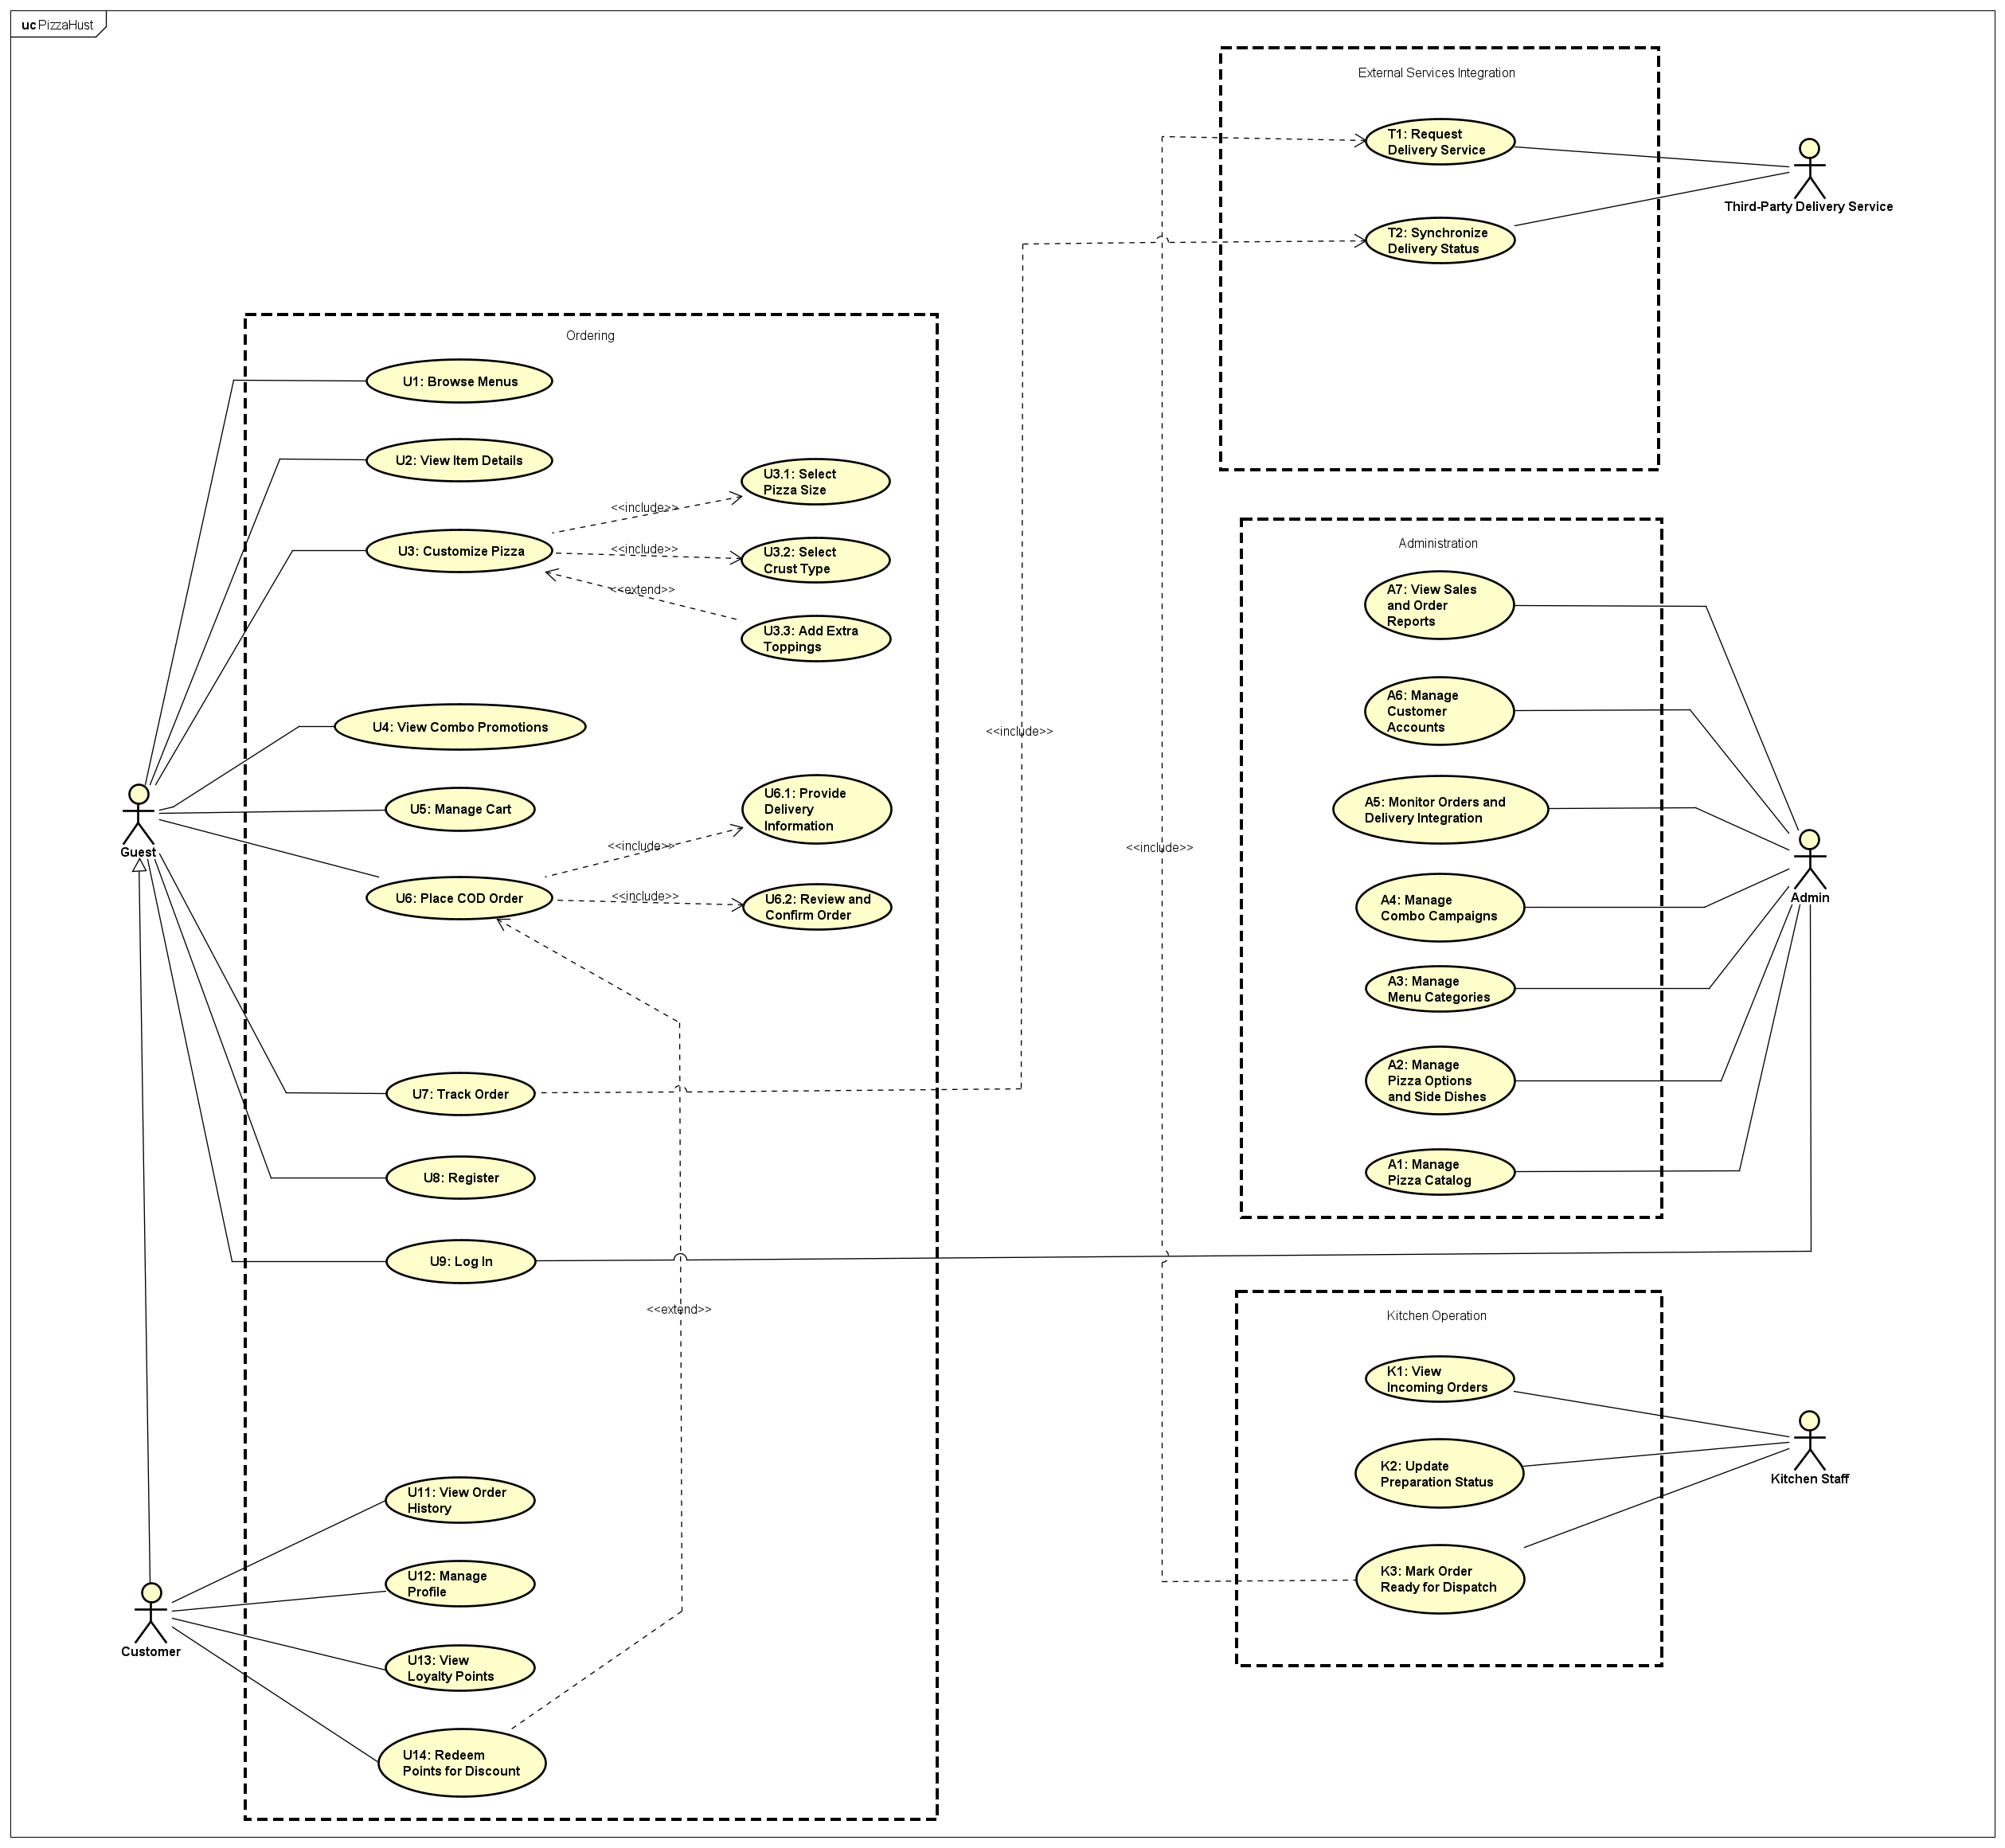
\includegraphics[width=\textwidth,height=0.86\textheight,keepaspectratio]{../PizzaHust.png}
    \caption{Overall use-case overview of PizzaHUST from the updated analysis artifact}
    \label{fig:use-case-overview}
\end{figure}

The overview shows four major interaction areas: customer ordering and account behavior, administrative management, kitchen operations, and delivery-service integration. These same areas later reappear in the architecture, database, API, and testing sections, which makes the use-case model the main bridge between requirements analysis and implementation evidence.

\subsection{Use-case relationships}

The use-case model is not a flat list of isolated actions. Several relationships are especially important:

\begin{itemize}
    \item \textbf{Actor generalization:} Customer extends Guest because authenticated users still perform the same public ordering actions.
    \item \textbf{Include relationships:} U6 \emph{Place COD Order} and U7 \emph{Track Order} depend on mandatory sub-behaviors such as delivery-information handling and delivery-state synchronization.
    \item \textbf{Extend relationships:} optional behaviors such as U14 \emph{Redeem Points for Discount} and U16 \emph{Add Order Notes} extend a base ordering flow rather than replacing it.
    \item \textbf{Operational interaction:} K3 \emph{Mark Order Ready for Dispatch} and A5 \emph{Monitor Orders and Delivery Exceptions} connect internal order handling with external delivery-service behavior T1 and T2.
\end{itemize}

\subsection{Detailed use case analysis}

This subsection presents the designed use-case set through a single consistent specification format. For readability, every use case is written as a bordered two-column table with the same fields: use-case code, use-case name, actor(s), brief description, preconditions, postconditions, basic flow of events, alternative flows of events, input data, and output data.

\setlength{\LTleft}{0pt}
\setlength{\LTright}{0pt}
\renewcommand{\arraystretch}{1.08}

\newcommand{\ucfield}[2]{\textbf{#1} & #2 \\ \hline}

\subsubsection*{Customer-facing use cases}

\begingroup
\footnotesize
\begin{longtable}{|>{\raggedright\arraybackslash}p{0.24\linewidth}|>{\raggedright\arraybackslash}p{0.70\linewidth}|}
\caption{Detailed use-case specification for U1: Browse Menus}\label{tab:uc-u1}\\ \hline
\textbf{Field} & \textbf{Description} \\ \hline
\endfirsthead
\caption[]{Detailed use-case specification for U1: Browse Menus (continued)}\\ \hline
\textbf{Field} & \textbf{Description} \\ \hline
\endhead
\ucfield{Use Case Code}{U1}
\ucfield{Use Case Name}{Browse Menus}
\ucfield{Actor(s)}{Guest, Customer}
\ucfield{Brief Description}{The user views active menu categories and products in order to find dishes available for ordering.}
\ucfield{Preconditions}{The system contains at least one active category and one active dish.}
\ucfield{Postconditions}{None. This is a read-only use case that may lead to U2 or U4.}
\ucfield{Basic Flow of Events}{1. The user opens the menu page. \newline 2. The system retrieves active categories and dishes. \newline 3. The system displays category filters and dish cards. \newline 4. The user changes the category filter. \newline 5. The system refreshes the visible menu list.}
\ucfield{Alternative Flows of Events}{1. If the selected category has no active dishes, the system shows an empty-category message. \newline 2. If the catalog request fails, the system shows an error state and a retry control.}
\ucfield{Input Data}{Optional category filter selected by the user.}
\ucfield{Output Data}{Active categories and visible dish cards.}
\end{longtable}
\endgroup

\begingroup
\footnotesize
\begin{longtable}{|>{\raggedright\arraybackslash}p{0.24\linewidth}|>{\raggedright\arraybackslash}p{0.70\linewidth}|}
\caption{Detailed use-case specification for U2: View Item Details}\label{tab:uc-u2}\\ \hline
\textbf{Field} & \textbf{Description} \\ \hline
\endfirsthead
\caption[]{Detailed use-case specification for U2: View Item Details (continued)}\\ \hline
\textbf{Field} & \textbf{Description} \\ \hline
\endhead
\ucfield{Use Case Code}{U2}
\ucfield{Use Case Name}{View Item Details}
\ucfield{Actor(s)}{Guest, Customer}
\ucfield{Brief Description}{The user opens a dish detail page to inspect product information and available customization options before ordering.}
\ucfield{Preconditions}{The selected dish exists and is active.}
\ucfield{Postconditions}{None. This is a read-only use case that may lead to U3 or U5.}
\ucfield{Basic Flow of Events}{1. The user selects a dish from the menu. \newline 2. The system retrieves the dish detail and enabled option groups. \newline 3. The system displays the dish name, image, base price, and customization entry point. \newline 4. The user reviews the information and decides whether to customize or add the item to the cart.}
\ucfield{Alternative Flows of Events}{1. If the dish becomes inactive after the menu page loads, the system reports that the item is no longer available. \newline 2. If the item is a simple side dish, the system hides pizza-specific customization controls.}
\ucfield{Input Data}{Selected dish identifier.}
\ucfield{Output Data}{Detailed item information and enabled option groups.}
\end{longtable}
\endgroup

\begingroup
\footnotesize
\begin{longtable}{|>{\raggedright\arraybackslash}p{0.24\linewidth}|>{\raggedright\arraybackslash}p{0.70\linewidth}|}
\caption{Detailed use-case specification for U3: Customize Pizza}\label{tab:uc-u3}\\ \hline
\textbf{Field} & \textbf{Description} \\ \hline
\endfirsthead
\caption[]{Detailed use-case specification for U3: Customize Pizza (continued)}\\ \hline
\textbf{Field} & \textbf{Description} \\ \hline
\endhead
\ucfield{Use Case Code}{U3}
\ucfield{Use Case Name}{Customize Pizza}
\ucfield{Actor(s)}{Guest, Customer}
\ucfield{Brief Description}{The user configures a pizza by selecting required and optional options, then obtains a server-validated quote before adding the line to the cart.}
\ucfield{Preconditions}{The target pizza is active and exposes the required option groups for customization.}
\ucfield{Postconditions}{A valid configured pizza line is ready to be added to the cart; no order is created yet.}
\ucfield{Basic Flow of Events}{1. The user opens the pizza customizer from the item detail page. \newline 2. The system shows enabled option groups such as size, crust, and toppings. \newline 3. The user selects required and optional options. \newline 4. The system sends the configuration to the quoting endpoint and returns the authoritative line total. \newline 5. The user confirms the configuration and proceeds to cart storage.}
\ucfield{Alternative Flows of Events}{1. If a selected option is no longer enabled, the system rejects the quote and asks the user to reselect. \newline 2. If a required group has no selection, the system blocks add-to-cart. \newline 3. If the dish becomes inactive during customization, the flow ends with an availability error.}
\ucfield{Input Data}{Selected option identifiers, optional dish note, and quantity.}
\ucfield{Output Data}{Server-computed line total and normalized selected-option summary.}
\end{longtable}
\endgroup

\begingroup
\footnotesize
\begin{longtable}{|>{\raggedright\arraybackslash}p{0.24\linewidth}|>{\raggedright\arraybackslash}p{0.70\linewidth}|}
\caption{Detailed use-case specification for U4: View Combo Promotions}\label{tab:uc-u4}\\ \hline
\textbf{Field} & \textbf{Description} \\ \hline
\endfirsthead
\caption[]{Detailed use-case specification for U4: View Combo Promotions (continued)}\\ \hline
\textbf{Field} & \textbf{Description} \\ \hline
\endhead
\ucfield{Use Case Code}{U4}
\ucfield{Use Case Name}{View Combo Promotions}
\ucfield{Actor(s)}{Guest, Customer}
\ucfield{Brief Description}{The user views active combo campaigns, including components, bundle pricing, and calculated savings.}
\ucfield{Preconditions}{At least one combo is active in the current validity window.}
\ucfield{Postconditions}{None. This is a read-only use case that may lead to U15.}
\ucfield{Basic Flow of Events}{1. The user opens the combo promotions page. \newline 2. The system retrieves currently active combos. \newline 3. The system displays each combo with name, components, price, and savings. \newline 4. The user opens a combo to inspect its details and possible customization path.}
\ucfield{Alternative Flows of Events}{1. If no combos are active, the system shows an empty state. \newline 2. If a combo is over-priced relative to its parts, the system still shows it but displays zero savings. \newline 3. If a combo expires while being viewed, the system blocks further ordering actions.}
\ucfield{Input Data}{Optional combo selected for detail viewing.}
\ucfield{Output Data}{Active combo list and combo detail information.}
\end{longtable}
\endgroup

\begingroup
\footnotesize
\begin{longtable}{|>{\raggedright\arraybackslash}p{0.24\linewidth}|>{\raggedright\arraybackslash}p{0.70\linewidth}|}
\caption{Detailed use-case specification for U5: Manage Cart}\label{tab:uc-u5}\\ \hline
\textbf{Field} & \textbf{Description} \\ \hline
\endfirsthead
\caption[]{Detailed use-case specification for U5: Manage Cart (continued)}\\ \hline
\textbf{Field} & \textbf{Description} \\ \hline
\endhead
\ucfield{Use Case Code}{U5}
\ucfield{Use Case Name}{Manage Cart}
\ucfield{Actor(s)}{Guest, Customer}
\ucfield{Brief Description}{The user reviews, edits, re-quotes, and removes intended order lines before proceeding to checkout.}
\ucfield{Preconditions}{A cart exists for the current guest session or authenticated customer session.}
\ucfield{Postconditions}{The cart reflects the latest valid user selections and authoritative pricing; no order is created yet.}
\ucfield{Basic Flow of Events}{1. The user opens the cart page. \newline 2. The system displays all cart lines with options, quantities, and line totals. \newline 3. The user edits quantity, configuration, or removes a line. \newline 4. The system re-quotes the cart and refreshes subtotal and discounts. \newline 5. The user proceeds to checkout.}
\ucfield{Alternative Flows of Events}{1. If a line's dish or combo becomes unavailable, the system flags that line for correction or removal. \newline 2. If a line contains an option no longer enabled for the dish, the system forces re-customization. \newline 3. If the cart is empty, checkout remains unavailable.}
\ucfield{Input Data}{Cart-line identifier, new quantity, or revised configuration.}
\ucfield{Output Data}{Updated line totals, subtotal, and combo-discount values.}
\end{longtable}
\endgroup

\begingroup
\footnotesize
\begin{longtable}{|>{\raggedright\arraybackslash}p{0.24\linewidth}|>{\raggedright\arraybackslash}p{0.70\linewidth}|}
\caption{Detailed use-case specification for U6: Place COD Order}\label{tab:uc-u6}\\ \hline
\textbf{Field} & \textbf{Description} \\ \hline
\endfirsthead
\caption[]{Detailed use-case specification for U6: Place COD Order (continued)}\\ \hline
\textbf{Field} & \textbf{Description} \\ \hline
\endhead
\ucfield{Use Case Code}{U6}
\ucfield{Use Case Name}{Place COD Order}
\ucfield{Actor(s)}{Guest, Customer}
\ucfield{Brief Description}{The user submits the cart as a cash-on-delivery order after delivery validation and final server-side order checking.}
\ucfield{Preconditions}{The cart contains at least one valid line; if loyalty redemption is used, the actor is an authenticated customer.}
\ucfield{Postconditions}{A new order is created with an order code and initial processing state; the order enters kitchen processing.}
\ucfield{Basic Flow of Events}{1. The user proceeds from the cart to checkout. \newline 2. The system displays the recipient and delivery form. \newline 3. The user enters recipient information, phone number, address, and optional delivery note. \newline 4. The system validates the address, applies the fixed delivery fee, and recalculates totals. \newline 5. The customer may optionally redeem loyalty points. \newline 6. The user confirms the COD purchase. \newline 7. The system revalidates all lines and persists the order with a generated code. \newline 8. The system shows the confirmation page and tracking entry point.}
\ucfield{Alternative Flows of Events}{1. If the address is outside the supported service area, the system rejects the address and blocks submission. \newline 2. If the phone number format is invalid, the system highlights the error. \newline 3. If a cart line becomes unavailable during final validation, the system returns the user to cart correction. \newline 4. If loyalty redemption exceeds the balance or cap, the system rejects that redemption.}
\ucfield{Input Data}{Recipient name, phone number, delivery address, optional delivery note, and optional redeemed points.}
\ucfield{Output Data}{Order code, persisted order summary, delivery fee, loyalty discount if any, and final COD total.}
\end{longtable}
\endgroup

\begingroup
\footnotesize
\begin{longtable}{|>{\raggedright\arraybackslash}p{0.24\linewidth}|>{\raggedright\arraybackslash}p{0.70\linewidth}|}
\caption{Detailed use-case specification for U7: Track Order}\label{tab:uc-u7}\\ \hline
\textbf{Field} & \textbf{Description} \\ \hline
\endfirsthead
\caption[]{Detailed use-case specification for U7: Track Order (continued)}\\ \hline
\textbf{Field} & \textbf{Description} \\ \hline
\endhead
\ucfield{Use Case Code}{U7}
\ucfield{Use Case Name}{Track Order}
\ucfield{Actor(s)}{Guest, Customer}
\ucfield{Brief Description}{The user follows order progress through a tracking view that exposes minimal public information for guests and richer detail for the owning customer.}
\ucfield{Preconditions}{The target order exists; guest tracking requires a valid order code.}
\ucfield{Postconditions}{None. This is a read-only use case.}
\ucfield{Basic Flow of Events}{1. The user opens the tracking page and provides the order code, or follows a direct tracking link. \newline 2. The system resolves the order and returns the visible tracking projection. \newline 3. The system displays the status timeline and promised delivery time. \newline 4. The tracking view continues polling for updates as the order progresses.}
\ucfield{Alternative Flows of Events}{1. If the order code is unknown, the system shows an order-not-found message. \newline 2. If lookup rate limits are exceeded, the system blocks further requests temporarily. \newline 3. If the order becomes cancelled or delivery-failed, the system shows the terminal state and ends tracking progression.}
\ucfield{Input Data}{Order code for guest lookup, or authenticated customer session for owned orders.}
\ucfield{Output Data}{Current status, status timeline, promised time, and privacy-filtered recipient information.}
\end{longtable}
\endgroup

\begingroup
\footnotesize
\begin{longtable}{|>{\raggedright\arraybackslash}p{0.24\linewidth}|>{\raggedright\arraybackslash}p{0.70\linewidth}|}
\caption{Detailed use-case specification for U8: Register Account}\label{tab:uc-u8}\\ \hline
\textbf{Field} & \textbf{Description} \\ \hline
\endfirsthead
\caption[]{Detailed use-case specification for U8: Register Account (continued)}\\ \hline
\textbf{Field} & \textbf{Description} \\ \hline
\endhead
\ucfield{Use Case Code}{U8}
\ucfield{Use Case Name}{Register Account}
\ucfield{Actor(s)}{Guest}
\ucfield{Brief Description}{A guest creates a customer account by submitting personal identification and login credentials.}
\ucfield{Preconditions}{The visitor is not currently authenticated.}
\ucfield{Postconditions}{A customer account exists and an authenticated session is started.}
\ucfield{Basic Flow of Events}{1. The guest opens the registration page. \newline 2. The system displays the registration form. \newline 3. The guest enters full name, phone number, password, and address. \newline 4. The system validates uniqueness and password rules. \newline 5. The system creates the account, starts the session, and redirects the user back into the storefront.}
\ucfield{Alternative Flows of Events}{1. If the phone number is already registered, the system rejects the registration. \newline 2. If the password does not satisfy the strength policy, the system highlights the rule violation. \newline 3. If registration rate limits are exceeded, the system temporarily rejects the request.}
\ucfield{Input Data}{Full name, phone number, password, and default address.}
\ucfield{Output Data}{Authenticated session and newly created customer profile.}
\end{longtable}
\endgroup

\begingroup
\footnotesize
\begin{longtable}{|>{\raggedright\arraybackslash}p{0.24\linewidth}|>{\raggedright\arraybackslash}p{0.70\linewidth}|}
\caption{Detailed use-case specification for U9: Log In}\label{tab:uc-u9}\\ \hline
\textbf{Field} & \textbf{Description} \\ \hline
\endfirsthead
\caption[]{Detailed use-case specification for U9: Log In (continued)}\\ \hline
\textbf{Field} & \textbf{Description} \\ \hline
\endhead
\ucfield{Use Case Code}{U9}
\ucfield{Use Case Name}{Log In}
\ucfield{Actor(s)}{Customer}
\ucfield{Brief Description}{A registered customer authenticates with phone number and password to access account-protected features.}
\ucfield{Preconditions}{The customer account exists and is not locked.}
\ucfield{Postconditions}{The customer is authenticated and can access account-based use cases.}
\ucfield{Basic Flow of Events}{1. The customer opens the login page and enters phone number and password. \newline 2. The system verifies the credentials against the stored password hash. \newline 3. The system starts an authenticated session and issues the CSRF protection token. \newline 4. The system merges any guest-session cart into the account cart and redirects the customer.}
\ucfield{Alternative Flows of Events}{1. If the credentials are invalid, the system shows a generic authentication error. \newline 2. If the account is locked by an administrator, the system refuses login. \newline 3. If login rate limits are exceeded, the system temporarily rejects the request.}
\ucfield{Input Data}{Registered phone number and password.}
\ucfield{Output Data}{Authenticated customer session and merged cart context if applicable.}
\end{longtable}
\endgroup

\begingroup
\footnotesize
\begin{longtable}{|>{\raggedright\arraybackslash}p{0.24\linewidth}|>{\raggedright\arraybackslash}p{0.70\linewidth}|}
\caption{Detailed use-case specification for U11: View Order History}\label{tab:uc-u11}\\ \hline
\textbf{Field} & \textbf{Description} \\ \hline
\endfirsthead
\caption[]{Detailed use-case specification for U11: View Order History (continued)}\\ \hline
\textbf{Field} & \textbf{Description} \\ \hline
\endhead
\ucfield{Use Case Code}{U11}
\ucfield{Use Case Name}{View Order History}
\ucfield{Actor(s)}{Customer}
\ucfield{Brief Description}{An authenticated customer views previous and current orders associated with their own account.}
\ucfield{Preconditions}{The customer is logged in.}
\ucfield{Postconditions}{None. This is a read-only use case that may lead to U7 for in-progress orders.}
\ucfield{Basic Flow of Events}{1. The customer opens the order history page. \newline 2. The system lists the customer's orders, newest first. \newline 3. The customer selects one order. \newline 4. The system shows complete order details, including lines, totals, and status timeline. \newline 5. The customer may jump to live tracking for an in-progress order.}
\ucfield{Alternative Flows of Events}{1. If the account has no orders, the system shows an empty state linking back to ordering. \newline 2. If the customer attempts to access an order belonging to another account, the system denies access.}
\ucfield{Input Data}{Customer session and selected order identifier.}
\ucfield{Output Data}{Paginated order list and full detail for the selected order.}
\end{longtable}
\endgroup

\begingroup
\footnotesize
\begin{longtable}{|>{\raggedright\arraybackslash}p{0.24\linewidth}|>{\raggedright\arraybackslash}p{0.70\linewidth}|}
\caption{Detailed use-case specification for U12: Manage Profile}\label{tab:uc-u12}\\ \hline
\textbf{Field} & \textbf{Description} \\ \hline
\endfirsthead
\caption[]{Detailed use-case specification for U12: Manage Profile (continued)}\\ \hline
\textbf{Field} & \textbf{Description} \\ \hline
\endhead
\ucfield{Use Case Code}{U12}
\ucfield{Use Case Name}{Manage Profile}
\ucfield{Actor(s)}{Customer}
\ucfield{Brief Description}{An authenticated customer edits profile information such as full name, default address, avatar, and password.}
\ucfield{Preconditions}{The customer is logged in.}
\ucfield{Postconditions}{The edited profile values are persisted; any supported credential change takes effect for later sessions.}
\ucfield{Basic Flow of Events}{1. The customer opens the profile page. \newline 2. The system displays current profile data with phone number treated as read-only. \newline 3. The customer edits supported profile fields and submits the form. \newline 4. The system validates and persists the changes. \newline 5. The customer may also upload an avatar or change password from the same account surface.}
\ucfield{Alternative Flows of Events}{1. If a field fails validation, the system rejects the update and highlights the problem. \newline 2. If an avatar upload fails type or size validation, the system rejects that file. \newline 3. If the current password is wrong during a password-change attempt, the system rejects the credential change.}
\ucfield{Input Data}{Edited profile fields, and in full scope optional avatar file or password-change data.}
\ucfield{Output Data}{Updated profile summary and confirmation feedback.}
\end{longtable}
\endgroup

\begingroup
\footnotesize
\begin{longtable}{|>{\raggedright\arraybackslash}p{0.24\linewidth}|>{\raggedright\arraybackslash}p{0.70\linewidth}|}
\caption{Detailed use-case specification for U13: View Loyalty Points}\label{tab:uc-u13}\\ \hline
\textbf{Field} & \textbf{Description} \\ \hline
\endfirsthead
\caption[]{Detailed use-case specification for U13: View Loyalty Points (continued)}\\ \hline
\textbf{Field} & \textbf{Description} \\ \hline
\endhead
\ucfield{Use Case Code}{U13}
\ucfield{Use Case Name}{View Loyalty Points}
\ucfield{Actor(s)}{Customer}
\ucfield{Brief Description}{An authenticated customer checks the current loyalty balance and the rules for earning and spending points.}
\ucfield{Preconditions}{The customer is logged in.}
\ucfield{Postconditions}{None. This is a read-only use case.}
\ucfield{Basic Flow of Events}{1. The customer opens the loyalty page or inspects the balance shown in the authenticated header. \newline 2. The system displays the current balance and the earning and redemption rules. \newline 3. The system shows the loyalty history for recent earn and redemption activity.}
\ucfield{Alternative Flows of Events}{If the balance is zero and there is no loyalty history, the system shows an explanatory empty state.}
\ucfield{Input Data}{Authenticated customer identity.}
\ucfield{Output Data}{Current loyalty balance, rule explanation, and loyalty history entries.}
\end{longtable}
\endgroup

\begingroup
\footnotesize
\begin{longtable}{|>{\raggedright\arraybackslash}p{0.24\linewidth}|>{\raggedright\arraybackslash}p{0.70\linewidth}|}
\caption{Detailed use-case specification for U14: Redeem Points for Discount}\label{tab:uc-u14}\\ \hline
\textbf{Field} & \textbf{Description} \\ \hline
\endfirsthead
\caption[]{Detailed use-case specification for U14: Redeem Points for Discount (continued)}\\ \hline
\textbf{Field} & \textbf{Description} \\ \hline
\endhead
\ucfield{Use Case Code}{U14}
\ucfield{Use Case Name}{Redeem Points for Discount}
\ucfield{Actor(s)}{Customer}
\ucfield{Brief Description}{During checkout, the customer converts loyalty points into a discount on the current order, subject to balance and percentage-cap rules.}
\ucfield{Preconditions}{The customer is logged in, has a positive balance, and already has a valid quoted cart in checkout.}
\ucfield{Postconditions}{A valid loyalty discount is applied to the current order quote, and the corresponding points are reserved when the order is created.}
\ucfield{Basic Flow of Events}{1. The customer opens the redemption control during checkout. \newline 2. The customer enters the number of points to redeem. \newline 3. The system verifies that the requested points do not exceed the balance and discount cap. \newline 4. The system recalculates the order quote with the loyalty discount applied. \newline 5. The customer continues the checkout flow.}
\ucfield{Alternative Flows of Events}{1. If the requested points exceed the available balance, the system rejects the request. \newline 2. If the requested discount exceeds the allowed percentage of the subtotal, the system rejects the request with a validation error. \newline 3. If the order is later cancelled or delivery fails, the reserved points are released back to the customer.}
\ucfield{Input Data}{Number of points to redeem.}
\ucfield{Output Data}{Applied loyalty discount, recalculated order total, and visible remaining balance.}
\end{longtable}
\endgroup

\begingroup
\footnotesize
\begin{longtable}{|>{\raggedright\arraybackslash}p{0.24\linewidth}|>{\raggedright\arraybackslash}p{0.70\linewidth}|}
\caption{Detailed use-case specification for U15: Customize Combo}\label{tab:uc-u15}\\ \hline
\textbf{Field} & \textbf{Description} \\ \hline
\endfirsthead
\caption[]{Detailed use-case specification for U15: Customize Combo (continued)}\\ \hline
\textbf{Field} & \textbf{Description} \\ \hline
\endhead
\ucfield{Use Case Code}{U15}
\ucfield{Use Case Name}{Customize Combo}
\ucfield{Actor(s)}{Guest, Customer}
\ucfield{Brief Description}{The user resolves combo choice slots into concrete products and configures any pizza items inside the combo before the system produces a final quoted combo line.}
\ucfield{Preconditions}{The combo is currently active and each choice slot has at least one eligible product.}
\ucfield{Postconditions}{A resolved combo line with authoritative pricing is ready for cart storage; no order is created yet.}
\ucfield{Basic Flow of Events}{1. The user opens the combo customizer from the combo detail page. \newline 2. The system displays fixed components and customer-choice slots, including surcharge information. \newline 3. The user resolves each slot by choosing concrete products. \newline 4. The user configures pizza-specific options inside the chosen products where needed. \newline 5. The system quotes the fully resolved combo line and shows the resulting charged total and savings. \newline 6. The user confirms the configuration.}
\ucfield{Alternative Flows of Events}{1. If a slot remains unresolved, the system blocks continuation. \newline 2. If the number of selected slot picks does not match the required quantity, the system asks for correction. \newline 3. If a picked product is invalid for the slot category or option rules fail, the system rejects the quote. \newline 4. If the combo leaves its active validity window, the system stops the ordering flow.}
\ucfield{Input Data}{Selected products for each slot, option selections for configurable items, optional dish notes, and quantity.}
\ucfield{Output Data}{Charged combo total, calculated savings, and a normalized resolved configuration summary.}
\end{longtable}
\endgroup

\begingroup
\footnotesize
\begin{longtable}{|>{\raggedright\arraybackslash}p{0.24\linewidth}|>{\raggedright\arraybackslash}p{0.70\linewidth}|}
\caption{Detailed use-case specification for U16: Add Order Notes}\label{tab:uc-u16}\\ \hline
\textbf{Field} & \textbf{Description} \\ \hline
\endfirsthead
\caption[]{Detailed use-case specification for U16: Add Order Notes (continued)}\\ \hline
\textbf{Field} & \textbf{Description} \\ \hline
\endhead
\ucfield{Use Case Code}{U16}
\ucfield{Use Case Name}{Add Order Notes}
\ucfield{Actor(s)}{Guest, Customer}
\ucfield{Brief Description}{The user adds free-text notes either for kitchen-side dish preparation or for courier-side delivery instructions.}
\ucfield{Preconditions}{The user is customizing a dish or combo line, or is filling the checkout delivery form.}
\ucfield{Postconditions}{Notes are stored in the appropriate audience-specific place: dish-level note or order-level delivery note.}
\ucfield{Basic Flow of Events}{1. The user writes an optional dish note during product customization. \newline 2. The system stores the note with that line and later shows it in cart and kitchen views. \newline 3. The user writes an optional delivery note during checkout. \newline 4. The system stores the delivery note with the order and reveals it only at the appropriate dispatch and tracking stages.}
\ucfield{Alternative Flows of Events}{1. If a note exceeds the length limit, the system truncates or rejects the excess input. \newline 2. If no notes are provided, the relevant note sections are simply omitted from later views.}
\ucfield{Input Data}{Free-text dish note and/or free-text delivery note.}
\ucfield{Output Data}{Persisted kitchen-facing note and courier-facing note associated with the correct entity.}
\end{longtable}
\endgroup

\subsubsection*{Administrative use cases}

\begingroup
\footnotesize
\begin{longtable}{|>{\raggedright\arraybackslash}p{0.24\linewidth}|>{\raggedright\arraybackslash}p{0.70\linewidth}|}
\caption{Detailed use-case specification for A1: Manage Pizza Catalog}\label{tab:uc-a1}\\ \hline
\textbf{Field} & \textbf{Description} \\ \hline
\endfirsthead
\caption[]{Detailed use-case specification for A1: Manage Pizza Catalog (continued)}\\ \hline
\textbf{Field} & \textbf{Description} \\ \hline
\endhead
\ucfield{Use Case Code}{A1}
\ucfield{Use Case Name}{Manage Pizza Catalog}
\ucfield{Actor(s)}{Admin / Store Owner}
\ucfield{Brief Description}{The administrator creates, edits, activates, deactivates, and imports pizza and side-dish records so the storefront reflects actual offerings.}
\ucfield{Preconditions}{The administrator is authenticated and target categories exist.}
\ucfield{Postconditions}{Catalog records are persisted and storefront visibility reflects the active state of each dish.}
\ucfield{Basic Flow of Events}{1. The administrator opens the catalog-management interface. \newline 2. The system lists existing dishes with key attributes and filters. \newline 3. The administrator creates a new dish or edits an existing one. \newline 4. The system displays the dish form and accepts the submitted values. \newline 5. The system validates and persists the dish. \newline 6. The administrator may optionally upload an image or perform CSV import operations.}
\ucfield{Alternative Flows of Events}{1. If the selected category is missing or inactive, the system rejects the save. \newline 2. If the uploaded image violates type or size rules, the system rejects the upload. \newline 3. If deactivation would break an active combo dependency, the system blocks that change until the combo is corrected.}
\ucfield{Input Data}{Dish name, kind, category, base price, active state, and optional image or CSV rows.}
\ucfield{Output Data}{Saved catalog entry, optional image URL, and optional import report.}
\end{longtable}
\endgroup

\begingroup
\footnotesize
\begin{longtable}{|>{\raggedright\arraybackslash}p{0.24\linewidth}|>{\raggedright\arraybackslash}p{0.70\linewidth}|}
\caption{Detailed use-case specification for A2: Manage Pizza Options and Side Dishes}\label{tab:uc-a2}\\ \hline
\textbf{Field} & \textbf{Description} \\ \hline
\endfirsthead
\caption[]{Detailed use-case specification for A2: Manage Pizza Options and Side Dishes (continued)}\\ \hline
\textbf{Field} & \textbf{Description} \\ \hline
\endhead
\ucfield{Use Case Code}{A2}
\ucfield{Use Case Name}{Manage Pizza Options and Side Dishes}
\ucfield{Actor(s)}{Admin / Store Owner}
\ucfield{Brief Description}{In the original analysis scope, the administrator managed pizza-option definitions and side-dish data through a dedicated use case. In the refined design, these responsibilities are absorbed by A1 and later option-management refinements.}
\ucfield{Preconditions}{The administrator is authenticated.}
\ucfield{Postconditions}{Option and side-dish data remain consistent with current catalog rules, even though the responsibility is distributed across refined administrative modules.}
\ucfield{Basic Flow of Events}{1. The administrator enters option or side-dish management. \newline 2. The system exposes the relevant editing surface. \newline 3. The administrator adds, edits, activates, or deactivates the target records. \newline 4. The system validates the changes and persists them so they affect ordering behavior.}
\ucfield{Alternative Flows of Events}{1. If an option configuration is invalid, the system rejects the update. \newline 2. If a side dish references invalid category data or conflicting values, the system blocks the save.}
\ucfield{Input Data}{Option definitions, side-dish attributes, and activation states.}
\ucfield{Output Data}{Updated option data and updated side-dish catalog records.}
\end{longtable}
\endgroup

\begingroup
\footnotesize
\begin{longtable}{|>{\raggedright\arraybackslash}p{0.24\linewidth}|>{\raggedright\arraybackslash}p{0.70\linewidth}|}
\caption{Detailed use-case specification for A3: Manage Menu Categories}\label{tab:uc-a3}\\ \hline
\textbf{Field} & \textbf{Description} \\ \hline
\endfirsthead
\caption[]{Detailed use-case specification for A3: Manage Menu Categories (continued)}\\ \hline
\textbf{Field} & \textbf{Description} \\ \hline
\endhead
\ucfield{Use Case Code}{A3}
\ucfield{Use Case Name}{Manage Menu Categories}
\ucfield{Actor(s)}{Admin / Store Owner}
\ucfield{Brief Description}{The administrator creates, renames, orders, and deactivates categories that organize menu browsing and scope later combo behavior.}
\ucfield{Preconditions}{The administrator is authenticated.}
\ucfield{Postconditions}{Category structure is persisted and storefront grouping reflects the latest valid configuration.}
\ucfield{Basic Flow of Events}{1. The administrator opens category management. \newline 2. The system lists categories with ordering and active state. \newline 3. The administrator creates or edits a category, including sort order or activation state. \newline 4. The system validates and saves the category definition.}
\ucfield{Alternative Flows of Events}{1. If the category name duplicates an existing category, the system rejects the save. \newline 2. If a deactivated category is still referenced by active business rules, the system preserves consistency and surfaces the dependent problem.}
\ucfield{Input Data}{Category name, sort order, and active flag.}
\ucfield{Output Data}{Updated category list used by storefront and administration views.}
\end{longtable}
\endgroup

\begingroup
\footnotesize
\begin{longtable}{|>{\raggedright\arraybackslash}p{0.24\linewidth}|>{\raggedright\arraybackslash}p{0.70\linewidth}|}
\caption{Detailed use-case specification for A4: Manage Combo Campaigns}\label{tab:uc-a4}\\ \hline
\textbf{Field} & \textbf{Description} \\ \hline
\endfirsthead
\caption[]{Detailed use-case specification for A4: Manage Combo Campaigns (continued)}\\ \hline
\textbf{Field} & \textbf{Description} \\ \hline
\endhead
\ucfield{Use Case Code}{A4}
\ucfield{Use Case Name}{Manage Combo Campaigns}
\ucfield{Actor(s)}{Admin / Store Owner}
\ucfield{Brief Description}{The administrator creates and edits promotional combo campaigns with validity windows, bundle price, optional target group, and component definitions.}
\ucfield{Preconditions}{The administrator is authenticated and valid component products or slot categories exist.}
\ucfield{Postconditions}{The combo definition is persisted and becomes visible to customers when its validity rules allow.}
\ucfield{Basic Flow of Events}{1. The administrator opens combo management. \newline 2. The system lists existing combos and derived campaign status. \newline 3. The administrator creates a new combo or edits an existing one. \newline 4. The system displays the combo form with pricing, timing, and component configuration. \newline 5. The administrator defines the components and saves the combo. \newline 6. The system validates the campaign and persists it.}
\ucfield{Alternative Flows of Events}{1. If the combo has too few component units, the system rejects the save. \newline 2. If component products or slot categories are invalid, the system blocks persistence. \newline 3. If the validity window is inconsistent, the system rejects the campaign definition.}
\ucfield{Input Data}{Combo name, price, validity window, target group size, component set, and optional image.}
\ucfield{Output Data}{Saved combo record, derived campaign status, and preview of customer-visible savings.}
\end{longtable}
\endgroup

\begingroup
\footnotesize
\begin{longtable}{|>{\raggedright\arraybackslash}p{0.24\linewidth}|>{\raggedright\arraybackslash}p{0.70\linewidth}|}
\caption{Detailed use-case specification for A5: Monitor Orders and Delivery Exceptions}\label{tab:uc-a5}\\ \hline
\textbf{Field} & \textbf{Description} \\ \hline
\endfirsthead
\caption[]{Detailed use-case specification for A5: Monitor Orders and Delivery Exceptions (continued)}\\ \hline
\textbf{Field} & \textbf{Description} \\ \hline
\endhead
\ucfield{Use Case Code}{A5}
\ucfield{Use Case Name}{Monitor Orders and Delivery Exceptions}
\ucfield{Actor(s)}{Admin / Store Owner}
\ucfield{Brief Description}{The administrator supervises order progression across statuses, inspects order details, retries failed delivery handoffs, and performs valid cancellation actions.}
\ucfield{Preconditions}{The administrator is authenticated and orders exist in the system.}
\ucfield{Postconditions}{Administrative interventions are recorded only when they are valid according to the order-state rules.}
\ucfield{Basic Flow of Events}{1. The administrator opens the order-monitoring view. \newline 2. The system lists orders, their statuses, and any delivery-exception alerts. \newline 3. The administrator opens a specific order for detail inspection. \newline 4. When appropriate, the administrator retries a dispatch handoff or cancels the order. \newline 5. The system validates the requested action and updates the order accordingly.}
\ucfield{Alternative Flows of Events}{1. If retry dispatch fails again, the order stays in an exception state and remains retryable. \newline 2. If the administrator requests an invalid state transition, the system rejects the action. \newline 3. If a cancellation is requested after the order has advanced beyond allowed states, the system blocks the cancellation.}
\ucfield{Input Data}{Selected order identifier and requested administrative action, such as retry or cancel.}
\ucfield{Output Data}{Updated order-monitor view, order detail, and revised order-state timeline where permitted.}
\end{longtable}
\endgroup

\begingroup
\footnotesize
\begin{longtable}{|>{\raggedright\arraybackslash}p{0.24\linewidth}|>{\raggedright\arraybackslash}p{0.70\linewidth}|}
\caption{Detailed use-case specification for A6: Manage Customer Accounts}\label{tab:uc-a6}\\ \hline
\textbf{Field} & \textbf{Description} \\ \hline
\endfirsthead
\caption[]{Detailed use-case specification for A6: Manage Customer Accounts (continued)}\\ \hline
\textbf{Field} & \textbf{Description} \\ \hline
\endhead
\ucfield{Use Case Code}{A6}
\ucfield{Use Case Name}{Manage Customer Accounts}
\ucfield{Actor(s)}{Admin / Store Owner}
\ucfield{Brief Description}{The administrator searches customer accounts, inspects customer details, and locks or unlocks accounts when operational control is needed.}
\ucfield{Preconditions}{The administrator is authenticated.}
\ucfield{Postconditions}{The target account's lock state is persisted and enforced during later authentication attempts.}
\ucfield{Basic Flow of Events}{1. The administrator opens customer-account management. \newline 2. The system lists customers and supports search or filtering. \newline 3. The administrator opens a customer record to inspect profile and summary information. \newline 4. The administrator locks or unlocks the account and optionally records a reason. \newline 5. The system saves the account-control change.}
\ucfield{Alternative Flows of Events}{1. If the search query finds no matching accounts, the system shows an empty result state. \newline 2. If the customer has in-progress orders at the moment of locking, the account is locked without cancelling those orders. \newline 3. Any later login attempt by the locked customer is rejected.}
\ucfield{Input Data}{Search query, target customer identifier, and optional lock reason.}
\ucfield{Output Data}{Customer list, customer detail view, and saved lock-state information.}
\end{longtable}
\endgroup

\begingroup
\footnotesize
\begin{longtable}{|>{\raggedright\arraybackslash}p{0.24\linewidth}|>{\raggedright\arraybackslash}p{0.70\linewidth}|}
\caption{Detailed use-case specification for A7: View Sales and Order Reports}\label{tab:uc-a7}\\ \hline
\textbf{Field} & \textbf{Description} \\ \hline
\endfirsthead
\caption[]{Detailed use-case specification for A7: View Sales and Order Reports (continued)}\\ \hline
\textbf{Field} & \textbf{Description} \\ \hline
\endhead
\ucfield{Use Case Code}{A7}
\ucfield{Use Case Name}{View Sales and Order Reports}
\ucfield{Actor(s)}{Admin / Store Owner}
\ucfield{Brief Description}{The administrator reviews management-level reporting information such as revenue, order-status distribution, best-selling items, and delivery outcome rate.}
\ucfield{Preconditions}{The administrator is authenticated and the selected reporting range is valid.}
\ucfield{Postconditions}{None. This is a read-only use case, though export actions may produce files.}
\ucfield{Basic Flow of Events}{1. The administrator opens the reporting page. \newline 2. The administrator selects a date range and aggregation level. \newline 3. The system calculates and displays the requested report metrics. \newline 4. The administrator may export the report in CSV form.}
\ucfield{Alternative Flows of Events}{1. If the chosen date range contains no orders, the system shows zero-value results and an empty-range note. \newline 2. If the start date is later than the end date, the system rejects the query range.}
\ucfield{Input Data}{Date range, aggregation mode, and optional export request.}
\ucfield{Output Data}{Revenue totals, order-status counts, ranked best-selling items, delivery-success metrics, and optional CSV export.}
\end{longtable}
\endgroup

\subsubsection*{Kitchen-operation use cases}

\begingroup
\footnotesize
\begin{longtable}{|>{\raggedright\arraybackslash}p{0.24\linewidth}|>{\raggedright\arraybackslash}p{0.70\linewidth}|}
\caption{Detailed use-case specification for K1: View Incoming Orders}\label{tab:uc-k1}\\ \hline
\textbf{Field} & \textbf{Description} \\ \hline
\endfirsthead
\caption[]{Detailed use-case specification for K1: View Incoming Orders (continued)}\\ \hline
\textbf{Field} & \textbf{Description} \\ \hline
\endhead
\ucfield{Use Case Code}{K1}
\ucfield{Use Case Name}{View Incoming Orders}
\ucfield{Actor(s)}{Kitchen Staff}
\ucfield{Brief Description}{Kitchen staff observe the prioritized queue of received and preparing orders so they can decide what to process next.}
\ucfield{Preconditions}{Kitchen staff is authenticated and the kitchen dashboard is available.}
\ucfield{Postconditions}{None. This is a read-only use case that may lead to K2.}
\ucfield{Basic Flow of Events}{1. Kitchen staff opens the kitchen dashboard. \newline 2. The system reads the prioritized kitchen queue and renders visible order cards. \newline 3. The system displays preparation-relevant information such as items, options, and dish notes. \newline 4. The queue keeps refreshing at the configured polling interval. \newline 5. Kitchen staff selects an order to begin processing.}
\ucfield{Alternative Flows of Events}{1. If the queue is empty, the system shows an empty state while continuing to poll. \newline 2. If an order is cancelled by an administrator while displayed, the queue removes it on refresh. \newline 3. If an order becomes overdue, the system raises its priority and highlights that condition.}
\ucfield{Input Data}{Authenticated kitchen session and optional selected order.}
\ucfield{Output Data}{Prioritized kitchen queue with order cards and preparation details.}
\end{longtable}
\endgroup

\begingroup
\footnotesize
\begin{longtable}{|>{\raggedright\arraybackslash}p{0.24\linewidth}|>{\raggedright\arraybackslash}p{0.70\linewidth}|}
\caption{Detailed use-case specification for K2: Update Preparation Status}\label{tab:uc-k2}\\ \hline
\textbf{Field} & \textbf{Description} \\ \hline
\endfirsthead
\caption[]{Detailed use-case specification for K2: Update Preparation Status (continued)}\\ \hline
\textbf{Field} & \textbf{Description} \\ \hline
\endhead
\ucfield{Use Case Code}{K2}
\ucfield{Use Case Name}{Update Preparation Status}
\ucfield{Actor(s)}{Kitchen Staff}
\ucfield{Brief Description}{Kitchen staff accept an order for preparation and update its preparation progress so that customer and admin views stay synchronized with kitchen reality.}
\ucfield{Preconditions}{Kitchen staff is authenticated and the target order is in a valid queue state for kitchen action.}
\ucfield{Postconditions}{The order state and preparation sub-stage accurately reflect the latest kitchen progress.}
\ucfield{Basic Flow of Events}{1. Kitchen staff selects an order from the queue. \newline 2. The system displays the full preparation detail for that order. \newline 3. Kitchen staff accepts the order or updates its preparation sub-stage. \newline 4. The system validates the state transition and persists the update. \newline 5. Tracking and administration views receive the revised status through their next refresh cycle.}
\ucfield{Alternative Flows of Events}{1. If another staff member has already accepted the order, the system rejects the second acceptance. \newline 2. If the order is cancelled between selection and update, the transition is rejected. \newline 3. If staff choose a lower-priority order, the system may request confirmation.}
\ucfield{Input Data}{Selected order identifier and target preparation sub-stage.}
\ucfield{Output Data}{Updated order state, updated preparation sub-stage, and recorded kitchen timestamps.}
\end{longtable}
\endgroup

\begingroup
\footnotesize
\begin{longtable}{|>{\raggedright\arraybackslash}p{0.24\linewidth}|>{\raggedright\arraybackslash}p{0.70\linewidth}|}
\caption{Detailed use-case specification for K3: Mark Order Ready for Dispatch}\label{tab:uc-k3}\\ \hline
\textbf{Field} & \textbf{Description} \\ \hline
\endfirsthead
\caption[]{Detailed use-case specification for K3: Mark Order Ready for Dispatch (continued)}\\ \hline
\textbf{Field} & \textbf{Description} \\ \hline
\endhead
\ucfield{Use Case Code}{K3}
\ucfield{Use Case Name}{Mark Order Ready for Dispatch}
\ucfield{Actor(s)}{Kitchen Staff}
\ucfield{Brief Description}{After preparation finishes, kitchen staff mark the order ready and the system attempts the delivery-service handoff as part of the same operational transition.}
\ucfield{Preconditions}{Kitchen staff is authenticated and the order is in the correct preparation state for dispatch handoff.}
\ucfield{Postconditions}{The order either advances into the ready-for-dispatch path with a delivery reference, or enters a controlled handoff-exception state.}
\ucfield{Basic Flow of Events}{1. Kitchen staff marks the prepared order as ready. \newline 2. The system reveals courier-facing delivery instructions if present. \newline 3. The system sends the booking request to the delivery-service integration. \newline 4. If the booking succeeds, the system stores the delivery reference and advances the order into dispatch progression. \newline 5. The order then awaits pickup confirmation from the provider or manual fallback handling.}
\ucfield{Alternative Flows of Events}{1. If the provider handoff fails or times out, the system records a retryable handoff exception instead of silently losing the transition. \newline 2. If the order is in the wrong state for this action, the system rejects the transition. \newline 3. If courier pickup confirmation does not arrive normally, the workflow continues through K4.}
\ucfield{Input Data}{Target order selected for dispatch handoff.}
\ucfield{Output Data}{New order status, optional delivery reference, and visible dispatch-handoff result.}
\end{longtable}
\endgroup

\begingroup
\footnotesize
\begin{longtable}{|>{\raggedright\arraybackslash}p{0.24\linewidth}|>{\raggedright\arraybackslash}p{0.70\linewidth}|}
\caption{Detailed use-case specification for K4: Confirm Pickup Fallback}\label{tab:uc-k4}\\ \hline
\textbf{Field} & \textbf{Description} \\ \hline
\endfirsthead
\caption[]{Detailed use-case specification for K4: Confirm Pickup Fallback (continued)}\\ \hline
\textbf{Field} & \textbf{Description} \\ \hline
\endhead
\ucfield{Use Case Code}{K4}
\ucfield{Use Case Name}{Confirm Pickup Fallback}
\ucfield{Actor(s)}{Kitchen Staff}
\ucfield{Brief Description}{Kitchen staff manually confirm courier pickup when the normal provider pickup-confirmation path is unavailable.}
\ucfield{Preconditions}{Kitchen staff is authenticated, the order is ready for dispatch, and the courier has physically taken the order.}
\ucfield{Postconditions}{The order enters the delivering state through a valid manual fallback transition.}
\ucfield{Basic Flow of Events}{1. Kitchen staff identifies that courier pickup occurred without a provider confirmation event. \newline 2. Kitchen staff triggers the manual pickup-confirmation action. \newline 3. The system requests confirmation for the fallback action. \newline 4. The system records the valid transition into the delivering state and attributes it to the kitchen actor. \newline 5. Tracking and administration views reflect the new state.}
\ucfield{Alternative Flows of Events}{1. If a provider pickup event arrives concurrently, the state machine accepts the first valid transition and ignores the duplicate. \newline 2. If the order is not actually ready for dispatch, the system rejects the action. \newline 3. If staff cancel the confirmation prompt, no state change occurs.}
\ucfield{Input Data}{Target order selected for manual pickup confirmation.}
\ucfield{Output Data}{Updated delivering status and corresponding timeline entry.}
\end{longtable}
\endgroup

\subsubsection*{External delivery-integration use cases}

\begingroup
\footnotesize
\begin{longtable}{|>{\raggedright\arraybackslash}p{0.24\linewidth}|>{\raggedright\arraybackslash}p{0.70\linewidth}|}
\caption{Detailed use-case specification for T1: Request Delivery Service}\label{tab:uc-t1}\\ \hline
\textbf{Field} & \textbf{Description} \\ \hline
\endfirsthead
\caption[]{Detailed use-case specification for T1: Request Delivery Service (continued)}\\ \hline
\textbf{Field} & \textbf{Description} \\ \hline
\endhead
\ucfield{Use Case Code}{T1}
\ucfield{Use Case Name}{Request Delivery Service}
\ucfield{Actor(s)}{Third-Party Delivery Service}
\ucfield{Brief Description}{PizzaHUST books an external courier for a prepared order through the delivery-provider API.}
\ucfield{Preconditions}{The order is in a valid pre-dispatch state and delivery-provider configuration is present.}
\ucfield{Postconditions}{On success, the order has a stored provider reference and advances into the delivery lifecycle; on failure, the system preserves a retryable handoff path.}
\ucfield{Basic Flow of Events}{1. The system builds the dispatch request from store and order data. \newline 2. The system calls the delivery-provider booking API. \newline 3. The provider accepts the booking and returns a delivery reference. \newline 4. PizzaHUST stores that reference and applies the associated order-state transition. \newline 5. Later courier lifecycle events continue through T2.}
\ucfield{Alternative Flows of Events}{1. If the provider is unreachable or times out, the booking fails and the order remains in a controlled exception state. \newline 2. If the provider rejects the booking for business reasons, the system handles it as a failed handoff rather than a silent partial success.}
\ucfield{Input Data}{Pickup address, drop-off address, order code, recipient details, and COD summary.}
\ucfield{Output Data}{Delivery-provider reference and resulting post-handoff order state.}
\end{longtable}
\endgroup

\begingroup
\footnotesize
\begin{longtable}{|>{\raggedright\arraybackslash}p{0.24\linewidth}|>{\raggedright\arraybackslash}p{0.70\linewidth}|}
\caption{Detailed use-case specification for T2: Synchronize Delivery Status}\label{tab:uc-t2}\\ \hline
\textbf{Field} & \textbf{Description} \\ \hline
\endfirsthead
\caption[]{Detailed use-case specification for T2: Synchronize Delivery Status (continued)}\\ \hline
\textbf{Field} & \textbf{Description} \\ \hline
\endhead
\ucfield{Use Case Code}{T2}
\ucfield{Use Case Name}{Synchronize Delivery Status}
\ucfield{Actor(s)}{Third-Party Delivery Service}
\ucfield{Brief Description}{The delivery provider pushes signed lifecycle events back to PizzaHUST so order-tracking and final delivery state remain synchronized with real courier progress.}
\ucfield{Preconditions}{A delivery booking already exists and webhook security configuration is active.}
\ucfield{Postconditions}{Valid provider events are mapped into internal state transitions exactly once, and duplicate or forged callbacks do not corrupt state.}
\ucfield{Basic Flow of Events}{1. The provider sends a webhook callback carrying reference, delivery state, and event identity. \newline 2. PizzaHUST verifies the callback signature. \newline 3. The system performs idempotency checks to avoid replay effects. \newline 4. The system resolves the target order by provider reference and maps the provider state into an internal order transition. \newline 5. The system applies the valid transition, records the timeline entry, and triggers any delivery-side loyalty effects.}
\ucfield{Alternative Flows of Events}{1. If the signature is invalid or missing, the callback is rejected. \newline 2. If the event is a duplicate, the system acknowledges it without reapplying the transition. \newline 3. If the provider reference is unknown or the transition is invalid for the current state, the system safely rejects or ignores the event.}
\ucfield{Input Data}{Delivery reference, provider state, event identifier, and signed webhook payload.}
\ucfield{Output Data}{Updated internal order status, recorded delivery timeline entry, and any exactly-once loyalty side effects.}
\end{longtable}
\endgroup

\clearpage
\section{User Stories}

\subsection{Role of user stories in the project}

Use cases describe interaction structure at analysis level, but they are not the most practical unit for incremental implementation planning. User stories complement the use-case model by expressing development goals from the actor's point of view in a concise form: \emph{As a <role>, I want <goal>, so that <benefit>}. In PizzaHUST, user stories help translate the designed full scope into smaller, testable pieces of work that can be implemented and verified iteratively.

For that reason, the stories below are organized by business epic rather than listed as a single flat backlog. Each story also retains a link to the related use-case ID so that the report can preserve traceability between requirement analysis, design, implementation, and testing.

\subsection{Story organization by epic}

The PizzaHUST backlog is organized into the following epics:

\begin{itemize}
    \item storefront browsing and product customization;
    \item cart, checkout, and order tracking;
    \item authentication, account, and loyalty;
    \item administrative catalog and promotions;
    \item administrative operations and reporting;
    \item kitchen operations and delivery coordination.
\end{itemize}

This epic structure mirrors the system decomposition used later in the architecture and component sections.

\subsection{Customer-facing stories}

\begingroup
\footnotesize
\setlength{\LTpre}{0.4em}
\setlength{\LTpost}{0.8em}
\begin{longtable}{L{0.10\linewidth} L{0.39\linewidth} L{0.28\linewidth} L{0.12\linewidth}}
\caption{Customer-facing user stories}\label{tab:customer-user-stories}\\
\toprule
\textbf{ID} & \textbf{User story} & \textbf{Acceptance criteria summary} & \textbf{Status} \\
\midrule
\endfirsthead
\caption[]{Customer-facing user stories (continued)}\\
\toprule
\textbf{ID} & \textbf{User story} & \textbf{Acceptance criteria summary} & \textbf{Status} \\
\midrule
\endhead
\bottomrule
\endfoot
\bottomrule
\endlastfoot
US-U1 & As a guest, I want to browse active menu categories and items so that I can discover what the store offers. & Active categories and items are shown; unavailable items are not presented as orderable. & Completed \\
US-U2 & As a guest, I want to view item details so that I can decide whether the product fits my needs before ordering. & Item detail view includes name, price context, and relevant customization information. & Completed \\
US-U3 & As a guest, I want to customize a pizza so that I can choose size, crust, and optional toppings before purchase. & Valid selections produce an authoritative quote; invalid combinations are rejected clearly. & Completed \\
US-U4 & As a guest, I want to view combo promotions so that I can compare bundle offers with regular ordering. & Active combos are visible during valid campaign periods. & Completed \\
US-U15 & As a guest, I want to customize combo contents where customer choice is allowed so that the combo matches my preferences. & Eligible selections are constrained by combo definition; invalid slot choices are rejected. & Completed \\
US-U5 & As a guest, I want to manage a cart so that I can review and revise my intended purchase before checkout. & Cart lines can be added, updated, or removed while keeping totals consistent. & Completed \\
US-U6 & As a guest, I want to place a COD order so that I can complete a purchase without online payment. & Valid checkout data creates an order code; unsupported addresses or invalid cart state block submission. & Completed \\
US-U7 & As a guest, I want to track my order by code so that I can see order progress after checkout. & Valid order codes return current status and timeline information. & Completed \\
US-U8 & As a guest, I want to register an account so that I can access customer-specific features later. & Valid registration data creates an account; invalid or duplicate data is rejected. & Completed \\
US-U9 & As a customer, I want to log in so that I can access profile and account-based features securely. & Correct credentials create a session; invalid credentials are rejected safely. & Completed \\
US-U11 & As a customer, I want to view my order history so that I can review previous purchases. & Only the customer's own orders are visible; historical data is preserved. & Completed \\
US-U12 & As a customer, I want to manage my profile so that my account information remains current for future orders. & Profile updates validate allowed fields and preserve account integrity. & Completed \\
US-U13 & As a customer, I want to view my loyalty information so that I can understand my current rewards balance. & Loyalty summary is visible only to the authenticated customer. & Completed \\
US-U14 & As a customer, I want to redeem loyalty points during checkout so that I can reduce my order cost. & Redemption follows business caps and available balance rules. & Completed \\
US-U16 & As a customer, I want to add order-related notes so that the store or courier can follow special handling instructions. & Dish notes and delivery notes are stored in the correct context and do not corrupt pricing or order creation. & Completed \\
\end{longtable}
\endgroup

\subsection{Staff-facing and integration stories}

\begingroup
\footnotesize
\setlength{\LTpre}{0.4em}
\setlength{\LTpost}{0.8em}
\begin{longtable}{L{0.10\linewidth} L{0.39\linewidth} L{0.28\linewidth} L{0.12\linewidth}}
\caption{Staff-facing and integration user stories}\label{tab:staff-user-stories}\\
\toprule
\textbf{ID} & \textbf{User story} & \textbf{Acceptance criteria summary} & \textbf{Status} \\
\midrule
\endfirsthead
\caption[]{Staff-facing and integration user stories (continued)}\\
\toprule
\textbf{ID} & \textbf{User story} & \textbf{Acceptance criteria summary} & \textbf{Status} \\
\midrule
\endhead
\bottomrule
\endfoot
\bottomrule
\endlastfoot
US-A1 & As an administrator, I want to manage pizza items so that the public menu reflects current offerings. & Item creation and modification preserve valid catalog data. & Completed \\
US-A2 & As an administrator, I want to manage options and side dishes so that customizable products can be maintained centrally. & Option rules remain valid and assignable to products. & Completed \\
US-A3 & As an administrator, I want to manage menu categories so that products remain organized for customers and staff. & Categories can be created and updated without breaking item organization. & Completed \\
US-A4 & As an administrator, I want to manage combo campaigns so that the store can run timed promotions. & Validity windows and combo definitions are validated before publication. & Completed \\
US-A5 & As an administrator, I want to monitor orders and dispatch exceptions so that operational problems can be identified and resolved. & Orders remain filterable and retryable only when business rules allow intervention. & Completed \\
US-A6 & As an administrator, I want to manage customer accounts so that I can inspect and control access when needed. & Customer search and account lock/unlock actions respect authorization and data integrity. & Completed \\
US-A7 & As an administrator, I want to view basic sales and order reports so that I can monitor store performance. & Report outputs provide summary information over selected time ranges. & Completed \\
US-K1 & As kitchen staff, I want to view incoming orders so that I know what must be prepared next. & Incoming work is visible in a form suitable for kitchen operation. & Completed \\
US-K2 & As kitchen staff, I want to update preparation status so that the order lifecycle reflects actual kitchen progress. & Only valid status transitions are accepted. & Completed \\
US-K3 & As kitchen staff, I want to mark orders ready for dispatch so that prepared orders can move to delivery handoff. & Dispatch handoff respects state-transition rules and integration outcomes. & Completed \\
US-K4 & As kitchen staff, I want a pickup-confirmation fallback so that dispatch can continue when provider confirmation is unavailable. & Manual fallback is allowed only in valid order states and preserves workflow consistency. & Completed \\
US-T1 & As the delivery service, I want to receive structured delivery requests so that I can accept dispatch work from PizzaHUST. & Delivery requests contain the required information for provider-side handling. & Completed \\
US-T2 & As the delivery service, I want to send signed status callbacks so that PizzaHUST can synchronize delivery progress safely. & Only valid authenticated callbacks can update delivery-related state. & Completed \\
\end{longtable}
\endgroup

\subsection{Traceability from stories to use cases}

User stories are most useful when they remain traceable to analysis and implementation artifacts. Table~\ref{tab:story-traceability} shows representative links between stories, use cases, system elements, and verification targets.

\begingroup
\footnotesize
\setlength{\LTpre}{0.4em}
\setlength{\LTpost}{0.8em}
\captionof{table}{Traceability examples from user stories to design and implementation}\label{tab:story-traceability}
\begin{tabular}{L{0.11\linewidth} L{0.16\linewidth} L{0.23\linewidth} L{0.18\linewidth} L{0.22\linewidth}}
\toprule
\textbf{Story} & \textbf{Use case} & \textbf{Implementation focus} & \textbf{UI/API anchor} & \textbf{Verification anchor} \\
\midrule
US-U3 & U3 Customize Pizza & Pricing and option validation & item detail UI and quote API & backend pricing/option tests and frontend item-flow tests \\
US-U6 & U6 Place COD Order & Checkout and order creation & checkout flow and order API & order-placement tests and smoke flow \\
US-U7 & U7 Track Order & Tracking projection and visibility rules & tracking UI and track API & tracking tests \\
US-A4 & A4 Manage Combo Campaigns & combo CRUD and validity logic & admin combo pages and combo APIs & admin combo tests \\
US-A5 & A5 Monitor Orders and Delivery Exceptions & order-state exception handling & admin orders view and retry-dispatch API & admin order-dispatch tests \\
US-K3 & K3 Mark Order Ready for Dispatch & preparation-to-dispatch transition & kitchen action UI/API & kitchen-action tests \\
US-T2 & T2 Synchronize Delivery Status & webhook validation and state sync & delivery webhook endpoint & delivery webhook tests \\
\bottomrule
\end{tabular}
\endgroup

All user stories listed above are part of the completed full scope of PizzaHUST, and the table is retained for traceability to use cases, implementation anchors, and tests.

\clearpage
\section{System Architecture}

\subsection{Architectural style}

PizzaHUST adopts a web-based client--server architecture. Its current implementation is best described as a \emph{modular monolith}: one frontend application delivers the user interface, one backend application exposes the business API and core workflow logic, and one relational database stores operational data. In addition, the project includes a separate delivery-mock service used to simulate an external courier platform during development and verification.

This architectural choice is deliberate. The business scope is broad enough to require clear separation between customer ordering, administration, kitchen operations, and external delivery integration, but the overall project remains small enough that splitting the core system into multiple business microservices would add unnecessary deployment, debugging, and coordination overhead. A modular monolith therefore provides a suitable compromise between simplicity and structured separation.

\subsection{Architecture rationale}

The original project constraints strongly influence the architecture:

\begin{itemize}
    \item the system targets a single pizza store rather than a large multi-branch enterprise;
    \item the first release is web-only and focused on a manageable academic MVP;
    \item the development timeline is limited;
    \item the team must support both customer-facing and staff-facing workflows;
    \item integration with a delivery provider is required, but a production provider environment may not always be available during development.
\end{itemize}

Under these constraints, a modular monolith offers several advantages:

\begin{itemize}
    \item business rules remain centralized, which is important for pricing, order-state transitions, and delivery coordination;
    \item frontend and backend teams can work in parallel with a contract-defined API;
    \item deployment remains feasible through a small Docker Compose stack;
    \item external delivery behavior can still be tested realistically by isolating the delivery mock as a separate network service.
\end{itemize}

In other words, PizzaHUST is \emph{not} a microservice platform. The delivery mock is separated only to exercise a real integration boundary; the core business system remains one backend application.

\subsection{Technology stack}

\begingroup
\small
\setlength{\LTpre}{0.4em}
\setlength{\LTpost}{0.8em}
\captionof{table}{Technology stack and architectural role}\label{tab:technology-stack}
\begin{tabular}{L{0.24\linewidth} L{0.70\linewidth}}
\toprule
\textbf{Layer} & \textbf{Technology and architectural role} \\
\midrule
Frontend & Next.js 16.2.4 with React 19.2.5, TypeScript 5.9.3, and Tailwind CSS 4.2.4 for the web UI. \\
Backend & Python 3.12 target with FastAPI for HTTP APIs, Pydantic for data validation, and SQLAlchemy 2.x for ORM-based persistence. \\
Database evolution & Alembic migrations maintain schema history and drift control. \\
Database engine & MySQL 8.4 stores operational business data. \\
API contract & OpenAPI is exported by the backend and used to generate TypeScript API types for the frontend. \\
Testing and quality gates & Ruff, mypy, import-linter, pytest, Vitest, Playwright, ESLint, and build checks are combined in the verification pipeline. \\
Local orchestration & Docker Compose coordinates the development/demo runtime stack. \\
\bottomrule
\end{tabular}
\endgroup

\subsection{Runtime topology}

Figure~\ref{fig:system-architecture} shows the runtime view used for local development and demonstration.

\begin{figure}[htbp]
    \centering
    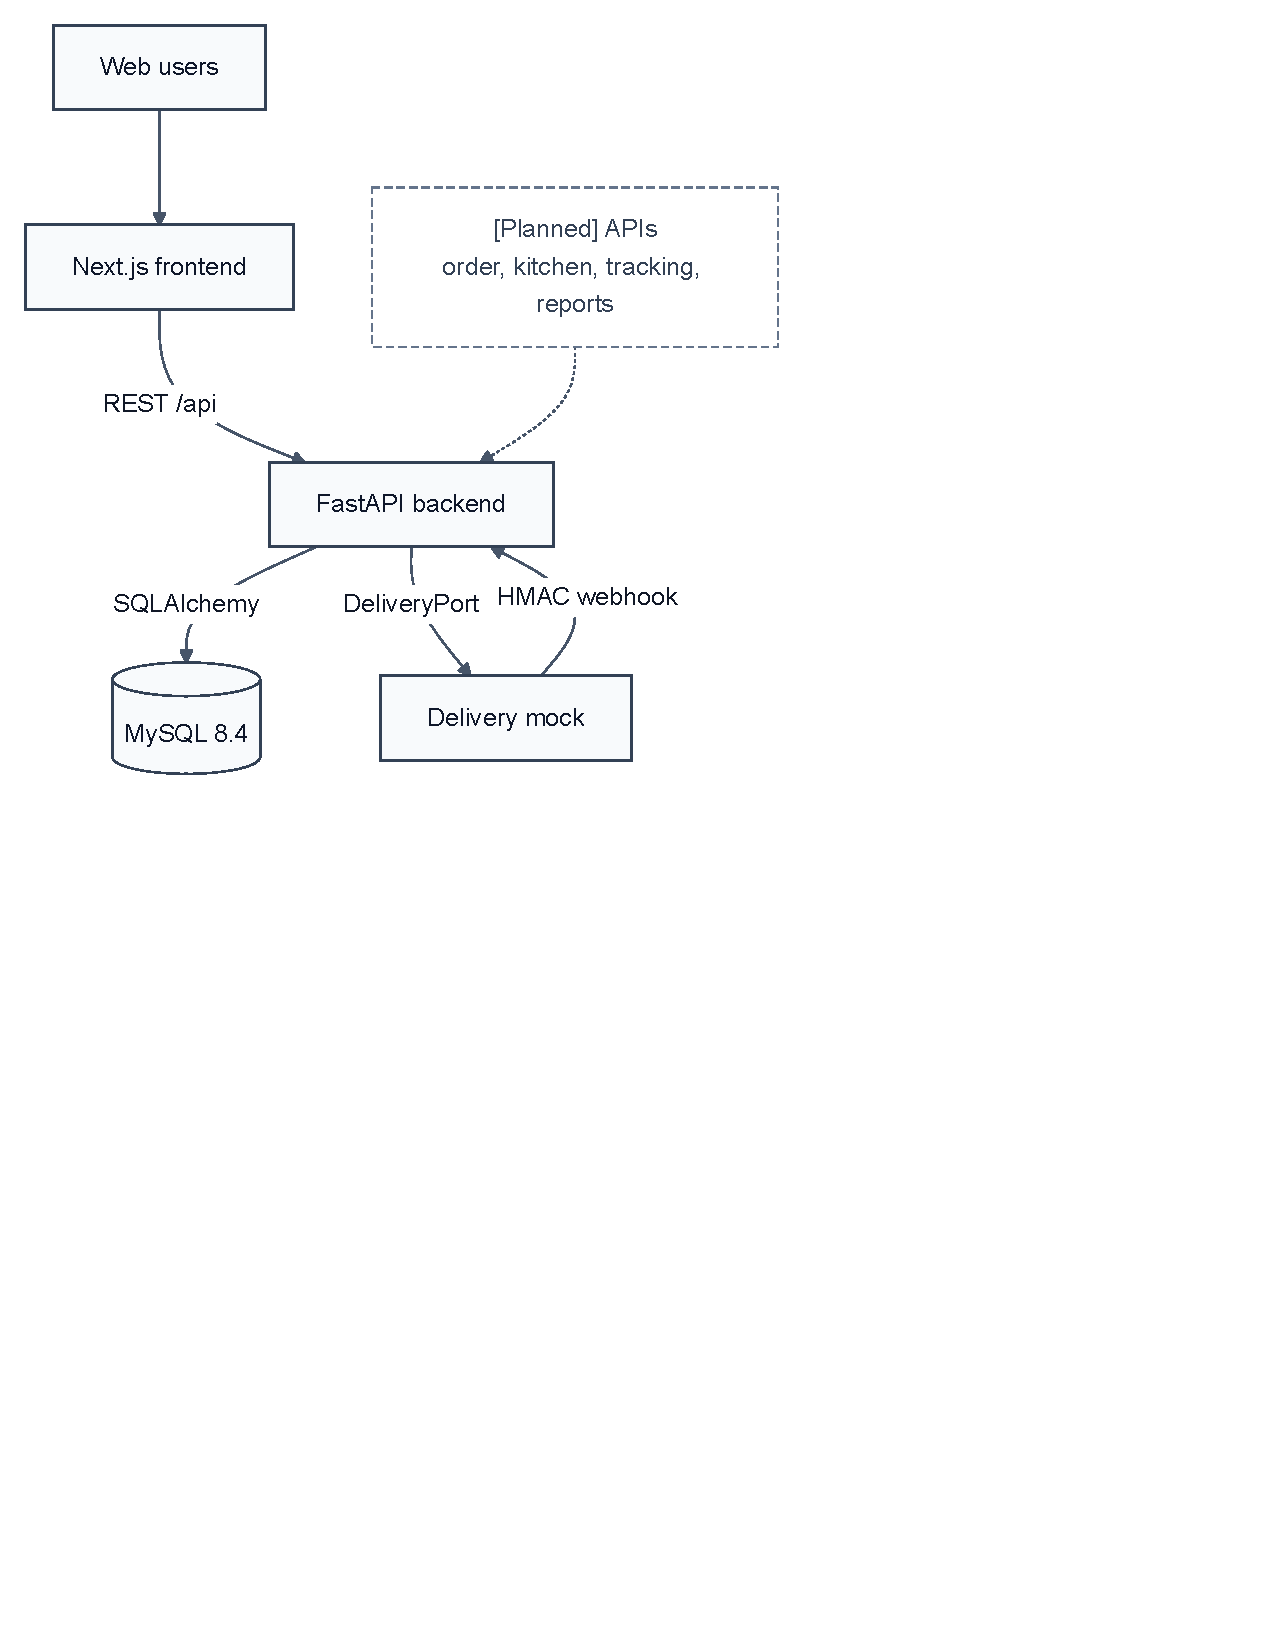
\includegraphics[width=0.86\textwidth,height=0.62\textheight,keepaspectratio,trim=8 410 230 8,clip]{latex_report/figures/system_architecture.pdf}
    \caption{Runtime architecture of PizzaHUST}
    \label{fig:system-architecture}
\end{figure}

The current Compose topology contains four runtime services:

\begin{itemize}
    \item \texttt{mysql}: the primary relational database, exposed internally on port 3306 and mapped to a configurable host port;
    \item \texttt{backend}: the FastAPI application, exposed on port 8000;
    \item \texttt{frontend}: the Next.js application, exposed on port 3000;
    \item \texttt{delivery-mock}: a separate FastAPI service exposed on port 9000 to simulate external courier integration.
\end{itemize}

All four services define health checks in the current development stack. This topology should be understood as a \emph{verified local/demo runtime environment}. The repository also contains infrastructure-oriented deployment assets, but the report should not claim that a production deployment topology has been fully validated solely from these local runtime checks.

\subsection{Backend boundary model}

The backend follows an explicit layered boundary model:

\begin{itemize}
    \item \texttt{app/api/}: HTTP entry points, request validation, response shaping, and orchestration of use-case-level actions;
    \item \texttt{app/domain/}: business rules such as pricing, option validation, combo logic, loyalty rules, service-area validation, and order-state transitions;
    \item \texttt{app/infra/}: persistence, configuration, authentication, and delivery-adapter support;
    \item \texttt{app/seeds/}: development and demo data generation.
\end{itemize}

This boundary model is not only descriptive; it is enforced by import-linter rules. Those rules forbid \texttt{app.domain} from importing API or infrastructure code and forbid \texttt{app.infra} from importing API code. This keeps business rules more testable and reduces coupling across layers.

At application startup, the backend registers routers for configuration, menu browsing, combos, cart behavior, order placement, order history, authentication, loyalty, administrative operations, kitchen operations, and delivery webhooks. This router composition reflects the system's use-case distribution and keeps each functional area addressable within the same API host.

\subsection{Security architecture}

The security model combines session-based authentication, request protection, and integration hardening.

\subsubsection{User authentication and authorization}

PizzaHUST uses Starlette session middleware with signed cookies for authenticated web access. Roles are modeled explicitly as \texttt{customer}, \texttt{admin}, and \texttt{kitchen}. Protected operations rely on role-check dependencies in the backend, while unauthenticated public routes remain available for browsing, quotation preview, and guest-facing actions where appropriate.

Passwords are hashed with Argon2. Mutating operations rely on CSRF protection through token handling, and login/register routes are rate-limited. This is an appropriate match for a browser-based monolithic web application where most state-changing operations originate from the project frontend.

\subsubsection{Delivery-integration security}

The delivery callback path uses HMAC validation and idempotent event recording. Incoming webhook requests must provide a valid signature before any state change is considered. Even for valid requests, repeated or duplicate events are handled safely through a stored webhook-event key. This is important because delivery synchronization is an external integration boundary and must not be trusted in the same way as internal UI actions.

\subsubsection{Request-level observability}

The backend assigns or propagates an \texttt{X-Request-ID} for incoming requests. This supports correlation across logs and responses and gives the API error envelope a stable request reference for troubleshooting.

\clearpage
\section{Component Architecture and Design}

\subsection{Design view and component boundaries}

The system architecture in the previous section explains the major runtime blocks. This section refines that view by describing how the application is decomposed into cooperating frontend, backend, persistence, and integration components. The goal of the component design is to keep each major responsibility understandable and testable while still supporting the end-to-end business flow of ordering, administration, kitchen processing, and delivery coordination.

Figure~\ref{fig:component-frontend} and Figure~\ref{fig:component-backend} summarize the main component organization currently reflected in the repository.

\begin{figure}[htbp]
    \centering
    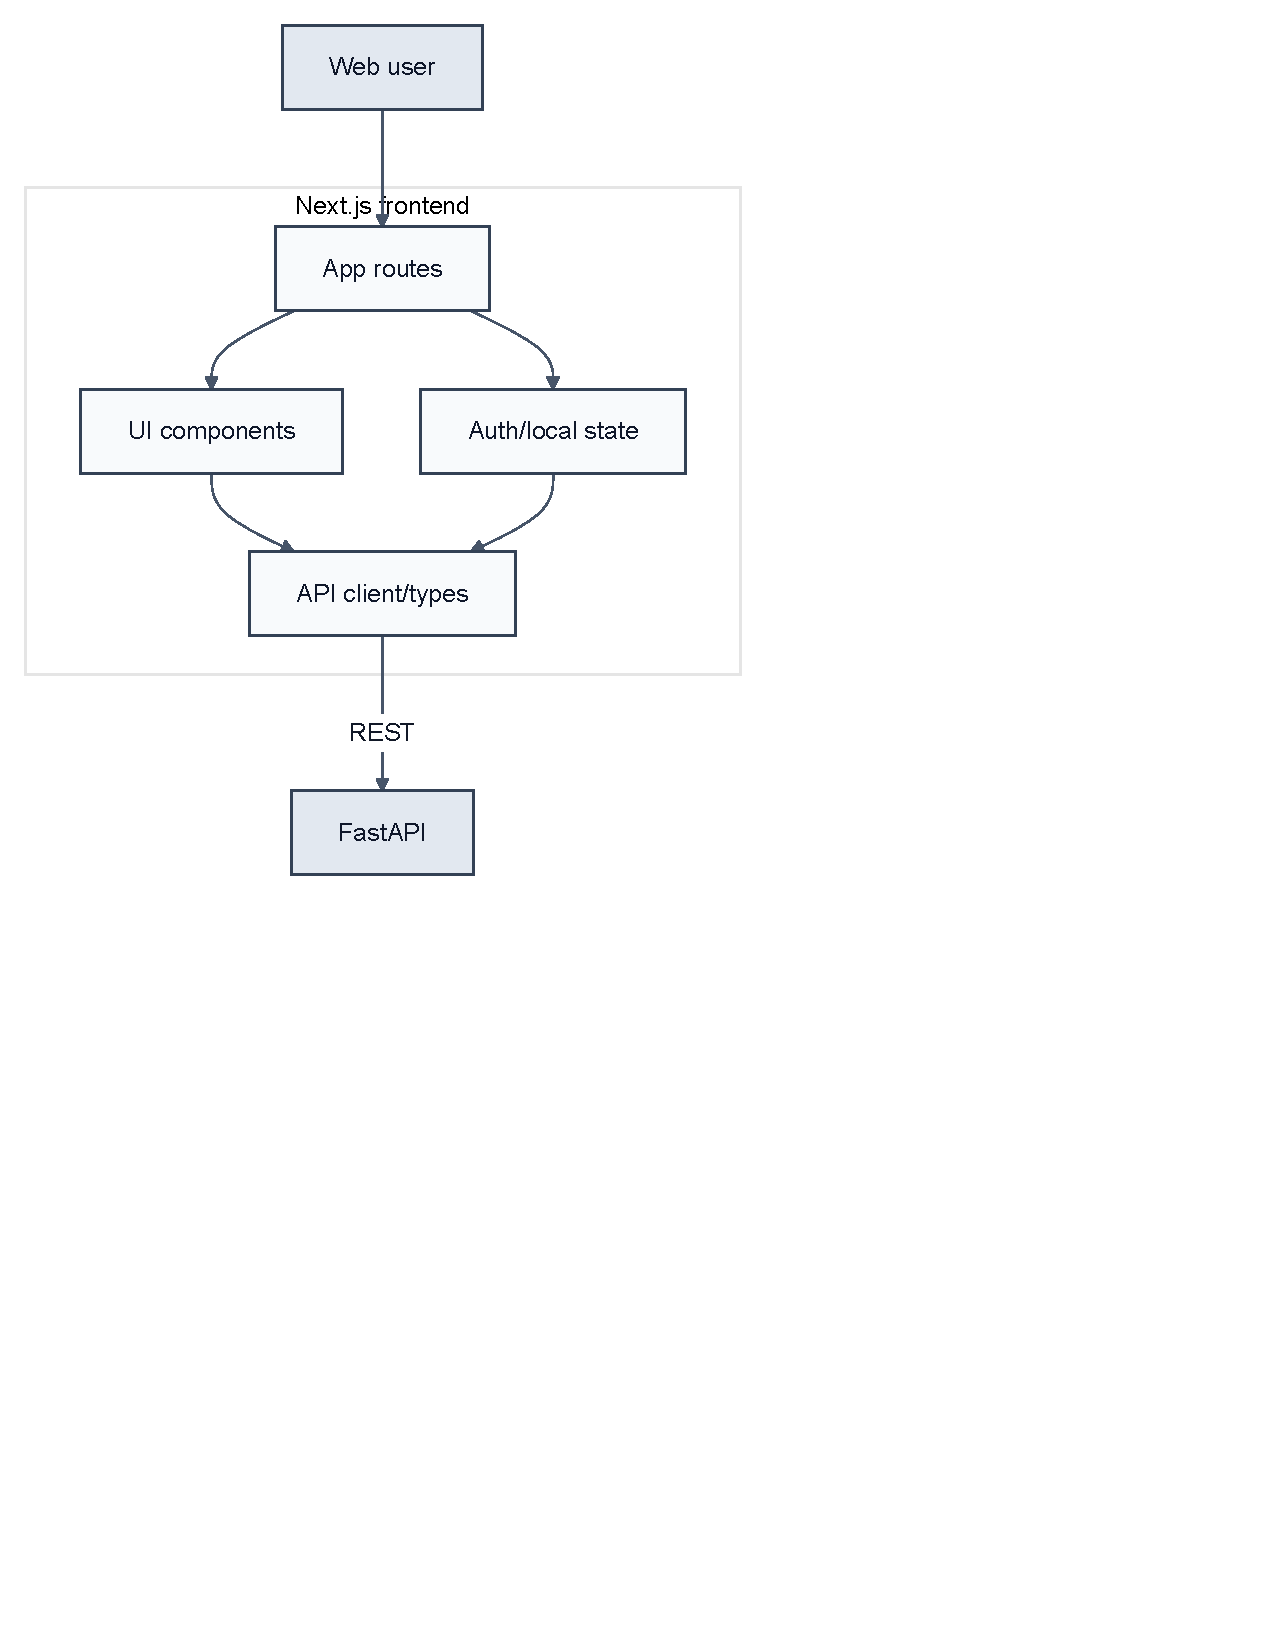
\includegraphics[width=0.78\textwidth,height=0.64\textheight,keepaspectratio,trim=8 367 252 8,clip]{latex_report/figures/component_frontend.pdf}
    \caption{Frontend component architecture}
    \label{fig:component-frontend}
\end{figure}

\begin{figure}[htbp]
    \centering
    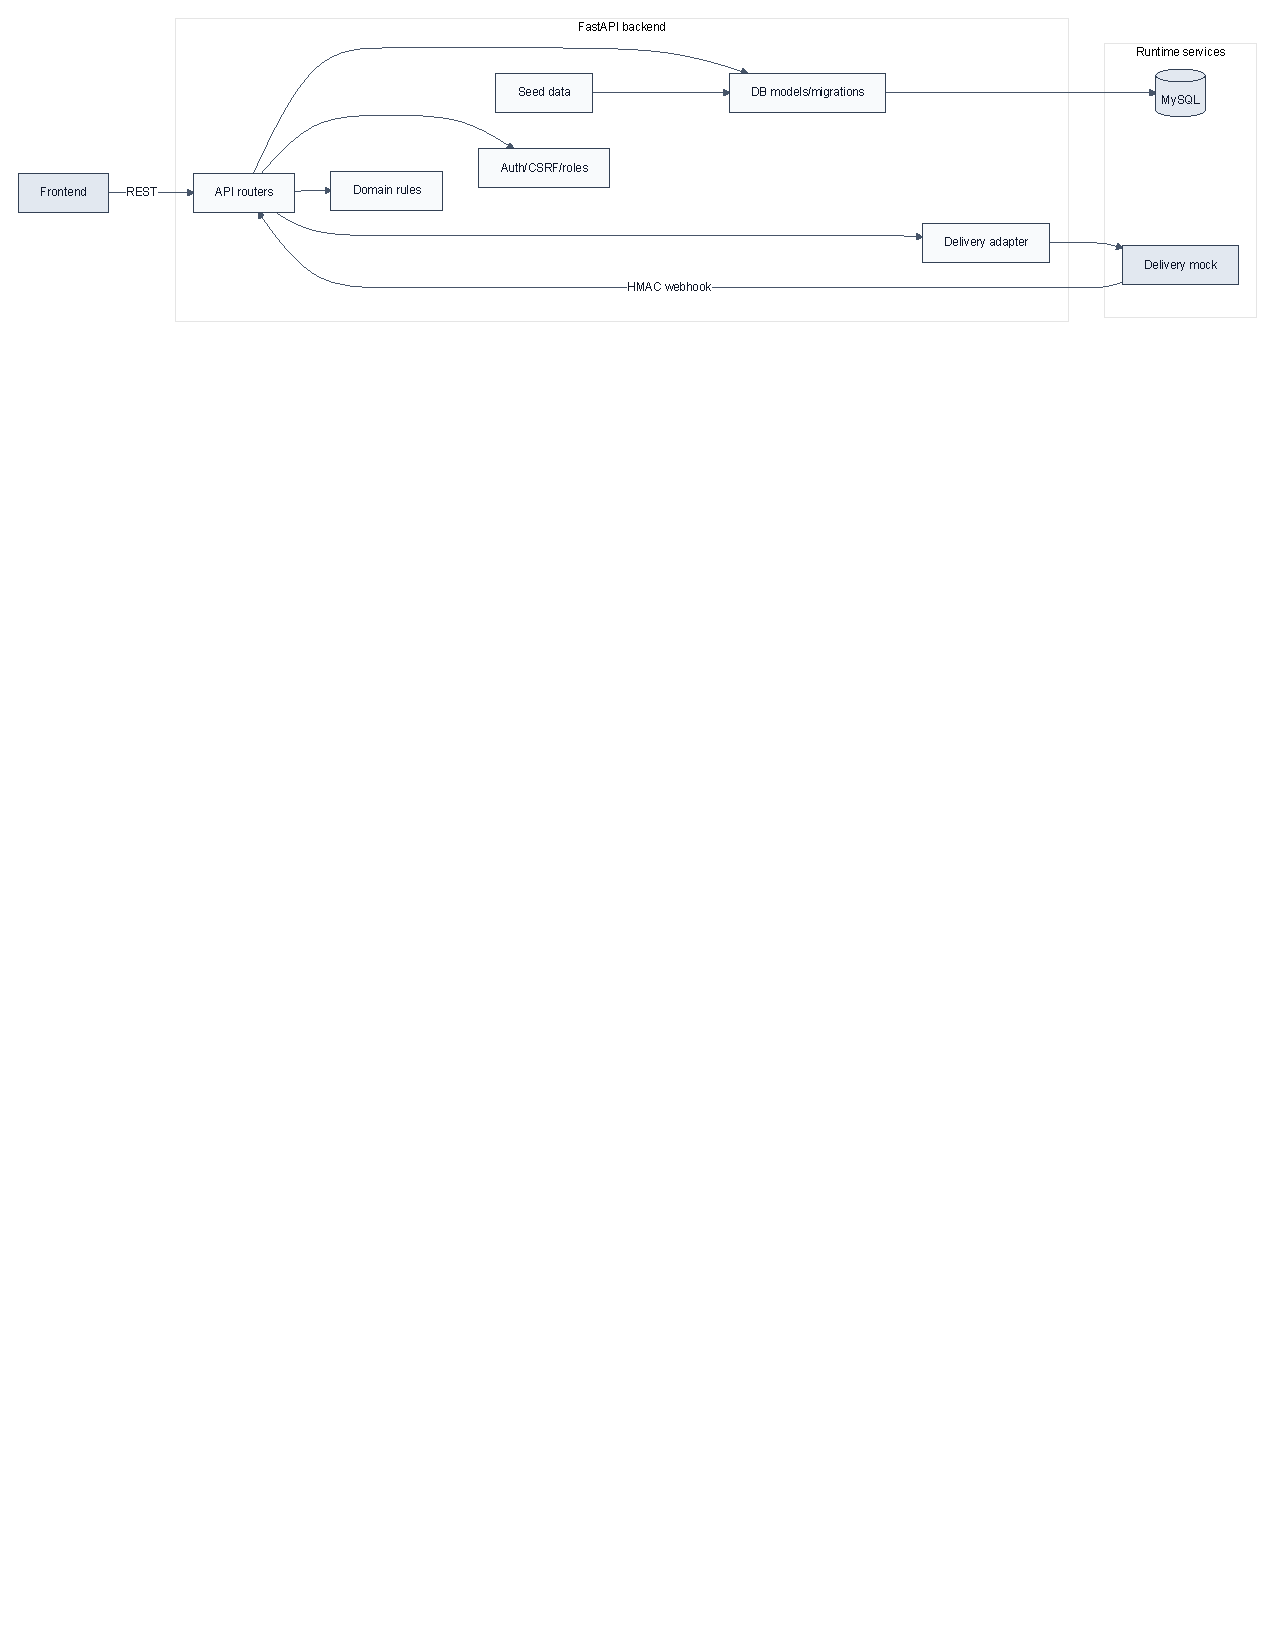
\includegraphics[width=0.95\textwidth,height=0.36\textheight,keepaspectratio,trim=6 632 6 6,clip]{latex_report/figures/component_backend.pdf}
    \caption{Backend and delivery component architecture}
    \label{fig:component-backend}
\end{figure}

\subsection{Frontend component architecture}

The frontend follows a route-plus-components structure centered on the Next.js App Router. Page routes own layout composition and page-level data loading, while reusable UI components encapsulate interaction logic for customer and staff workflows.

\begingroup
\small
\setlength{\LTpre}{0.4em}
\setlength{\LTpost}{0.8em}
\captionof{table}{Frontend component groups}\label{tab:frontend-components}
\begin{tabular}{L{0.19\linewidth} L{0.34\linewidth} L{0.39\linewidth}}
\toprule
\textbf{Component group} & \textbf{Main responsibility} & \textbf{Representative elements} \\
\midrule
Route components & Compose page-level UI, load data, and connect user interaction to feature APIs. & \texttt{app/menu/page.tsx}, \texttt{app/combos/[id]/page.tsx}, \texttt{app/admin/orders/page.tsx}, \texttt{app/kitchen/page.tsx} \\
Public shell components & Provide shared customer-facing navigation, layout chrome, footer, and theme handling. & \texttt{components/app-chrome.tsx}, \texttt{components/top-nav.tsx}, \texttt{components/site-footer.tsx} \\
Menu and product components & Render menu filtering, product cards, option selection, quantity controls, and item-detail UI. & \texttt{components/menu/*} \\
Combo components & Support combo cards, slot picking, step-based combo customization, and quote display. & \texttt{components/combos/*} \\
Administrator components & Support editing, searching, navigation, and management workflows for store operations. & \texttt{components/admin/*} \\
Shared state and auth & Provide session refresh and account-aware UI behavior. & \texttt{components/auth-provider.tsx}, cart provider, theme bootstrap \\
Frontend API layer & Encapsulate fetch behavior, credentials, CSRF injection, typed wrappers, and API error reporting. & \texttt{lib/api/client.ts}, \texttt{lib/api/menu.ts}, \texttt{lib/api/cart.ts}, \texttt{lib/api/admin-*} \\
\bottomrule
\end{tabular}
\endgroup

The frontend is intentionally componentized around business surfaces rather than only around visual primitives. For example, menu customization, combo customization, and administrator editors each have their own specialized component families because they orchestrate different workflow rules even when they share styling conventions.

\subsection{Backend component architecture}

The backend component design mirrors the layered architecture discussed earlier, but it is useful to restate it here in workflow terms.

\begingroup
\small
\setlength{\LTpre}{0.4em}
\setlength{\LTpost}{0.8em}
\captionof{table}{Backend component groups}\label{tab:backend-components}
\begin{tabular}{L{0.19\linewidth} L{0.34\linewidth} L{0.39\linewidth}}
\toprule
\textbf{Component group} & \textbf{Main responsibility} & \textbf{Representative modules} \\
\midrule
Public API routers & Expose catalog browsing, combo browsing, quotation, cart, and order functions. & \texttt{app/api/menu.py}, \texttt{app/api/combos.py}, \texttt{app/api/cart.py}, \texttt{app/api/orders.py} \\
Authentication and account routers & Handle registration, login, session inspection, profile updates, and loyalty access. & \texttt{app/api/auth.py}, \texttt{app/api/loyalty.py}, order-history endpoints \\
Administrative routers & Expose management actions for items, categories, option groups, combos, customers, orders, reports, import, and settings. & \texttt{app/api/admin/*} \\
Kitchen routers & Support kitchen-facing queue inspection and state-changing operational actions. & \texttt{app/api/kitchen/orders.py}, \texttt{app/api/kitchen/actions.py} \\
Integration router & Accept externally initiated delivery callbacks. & \texttt{app/api/webhooks.py} \\
Domain components & Enforce pricing, options, combos, service-area, loyalty, and order-state business logic. & \texttt{app/domain/*} \\
Persistence and support infrastructure & Provide ORM models, DB sessions, migrations, auth helpers, settings access, and delivery-adapter wiring. & \texttt{app/infra/db/*}, \texttt{app/infra/auth/*}, \texttt{app/infra/delivery/*} \\
External-provider simulator & Behave as a realistic network-visible courier system during development and testing. & \texttt{delivery\_mock/main.py} \\
\bottomrule
\end{tabular}
\endgroup

\subsection{Data and integration support components}

Not all important components are visible directly in the UI or API layer. Several supporting components are critical to the overall design:

\begin{itemize}
    \item the SQLAlchemy model layer, which defines durable business state and relationships;
    \item the migration layer, which preserves schema evolution through versioned changes;
    \item the settings service, which centralizes configurable values such as business timezone, loyalty parameters, and delivery fee mapping;
    \item the delivery-port abstraction, which isolates delivery-provider behavior from core order workflows;
    \item the generated OpenAPI contract and TypeScript types, which connect backend response models to frontend usage safely.
\end{itemize}

These support components are important because they reduce duplication of business rules and make cross-layer behavior more consistent.

\subsection{Component interaction scenarios}

\subsubsection{Pizza quotation flow}

When a customer opens an item-detail page, the route component loads product information and exposes option-selection controls through menu components. User choices are then packaged by the frontend API layer and sent to the quotation endpoint. On the backend, the cart quote router resolves the current product and enabled options from persistence, validates the selection through the options domain, and calculates totals through the pricing domain before returning an authoritative quote.

\subsubsection{Combo customization flow}

Combo customization involves a richer interaction path. The frontend combo customizer presents fixed components and category-scoped choice slots. The backend resolves combo definitions, validates slot selections, calculates any surcharge relative to the slot reference product, and combines that with option-delta pricing. This scenario shows why combo-related logic is not just a variant of simple product pricing.

\subsubsection{Administrative combo editing flow}

In the administrative interface, a combo editor page coordinates multiple component families: basic form controls, component pickers, image handling, and API mutation calls. The backend administrative combo router validates date ranges, component structure, and category-slot constraints before persistence. This interaction demonstrates how the system separates staff-facing CRUD orchestration from reusable domain rules.

\subsubsection{Delivery callback flow}

The delivery callback flow crosses the clearest system boundary. The delivery mock sends an HMAC-signed HTTP callback to the webhook router. The backend verifies the signature, enforces idempotency, maps the provider event to an internal order-state transition, and records a tracking entry. This scenario shows how integration logic, domain rules, persistence, and workflow history cooperate without requiring direct user interaction.

\subsection{Design rationale}

The component design of PizzaHUST follows three consistent principles:

\begin{itemize}
    \item \textbf{business-oriented decomposition:} components are grouped around meaningful workflows such as customization, administration, kitchen actions, and delivery integration;
    \item \textbf{separation of orchestration from rules:} routers and pages coordinate actions, while domain modules enforce reusable business logic;
    \item \textbf{support for incremental delivery:} the design allows some components to be implemented or refined earlier than others without collapsing the whole structure.
\end{itemize}

The current codebase is not perfectly uniform in every frontend data-access pattern, especially in some administrative pages, but the dominant structure is consistent enough to support maintainability and verification. For the scope of an academic project, this is a sound component design outcome.

\clearpage
\section{Database Design}

\subsection{Database design goals}

The PizzaHUST database is designed to support the complete business lifecycle of the system: user identity, catalog management, customization options, combo promotions, cart persistence, order creation, order tracking, kitchen prioritization, reporting support, and external-delivery synchronization. In practical terms, the schema must support both the \emph{designed full scope} of the project and the \emph{current implementation reality} captured in the repository.

Two database design requirements are especially important:

\begin{itemize}
    \item the schema must represent both guest orders and registered-customer orders;
    \item the schema must preserve historical order meaning even when live catalog data changes later.
\end{itemize}

These requirements explain several later design decisions, especially nullable user ownership on orders and snapshot storage for selected options.

\subsection{Conceptual ERD and evolved implementation schema}

The project includes an early DBML design derived from the Week 1 ERD and data-dictionary work. That early model captures the main business entities, but the implemented schema has evolved through migrations as the project moved from initial analysis to runnable application behavior.

This distinction matters for the report:

\begin{itemize}
    \item the DBML and early ERD describe the \emph{initial conceptual structure};
    \item the SQLAlchemy models and Alembic migrations describe the \emph{current evolved schema};
    \item the final report should acknowledge that the schema evolved, then present ERD figures regenerated from the current logical design rather than from the outdated draft alone.
\end{itemize}

For example, the current codebase includes category-owned option groups, combo choice slots, cart persistence, webhook idempotency, image galleries, loyalty accrual fields, tracking-note sources, and operational settings tables that do not all appear in the initial DBML snapshot.

\subsection{Entity groups and relationships}

Table~\ref{tab:database-entities} summarizes the main entity groups in the current design.

\begingroup
\small
\setlength{\LTpre}{0.4em}
\setlength{\LTpost}{0.8em}
\captionof{table}{Database entity groups and design purpose}\label{tab:database-entities}
\begin{tabular}{L{0.19\linewidth} L{0.35\linewidth} L{0.38\linewidth}}
\toprule
\textbf{Entity group} & \textbf{Main tables} & \textbf{Purpose} \\
\midrule
Identity and roles & \texttt{users} & Stores customer, admin, and kitchen identities, phone-based login data, profile data, roles, and loyalty totals. \\
Catalog structure & \texttt{categories}, \texttt{products}, \texttt{product\_images} & Organizes products, pricing baselines, activation state, and gallery images. \\
Customization model & \texttt{option\_groups}, \texttt{options}, \texttt{product\_options} & Defines reusable option groups and per-product option enablement. \\
Combo model & \texttt{combos}, \texttt{combo\_items}, \texttt{combo\_images} & Represents promotional bundles, timing windows, choice slots, and combo imagery. \\
Cart model & \texttt{carts}, \texttt{cart\_lines} & Stores server-side cart state for guest or authenticated users. \\
Order model & \texttt{orders}, \texttt{order\_items}, \texttt{order\_item\_options} & Stores placed orders, line items, combo decomposition, and historical selection snapshots. \\
Tracking and workflow audit & \texttt{order\_tracking}, \texttt{webhook\_events} & Records order-state history and protects delivery callbacks against duplicate processing. \\
Operational read/support data & \texttt{kitchen\_queue\_view}, \texttt{business\_settings}, \texttt{delivery\_ward\_fees} & Supports kitchen prioritization and configurable runtime business values. \\
\bottomrule
\end{tabular}
\endgroup

\subsection{Relationship overview}

To keep the schema readable in the report, the current database design is shown through one complete logical ERD and several smaller focused ERD views. The first figure gives full-schema coverage, while the later figures isolate the catalog/option model, the combo model, and the order/workflow model.

\begin{figure}[htbp]
    \centering
    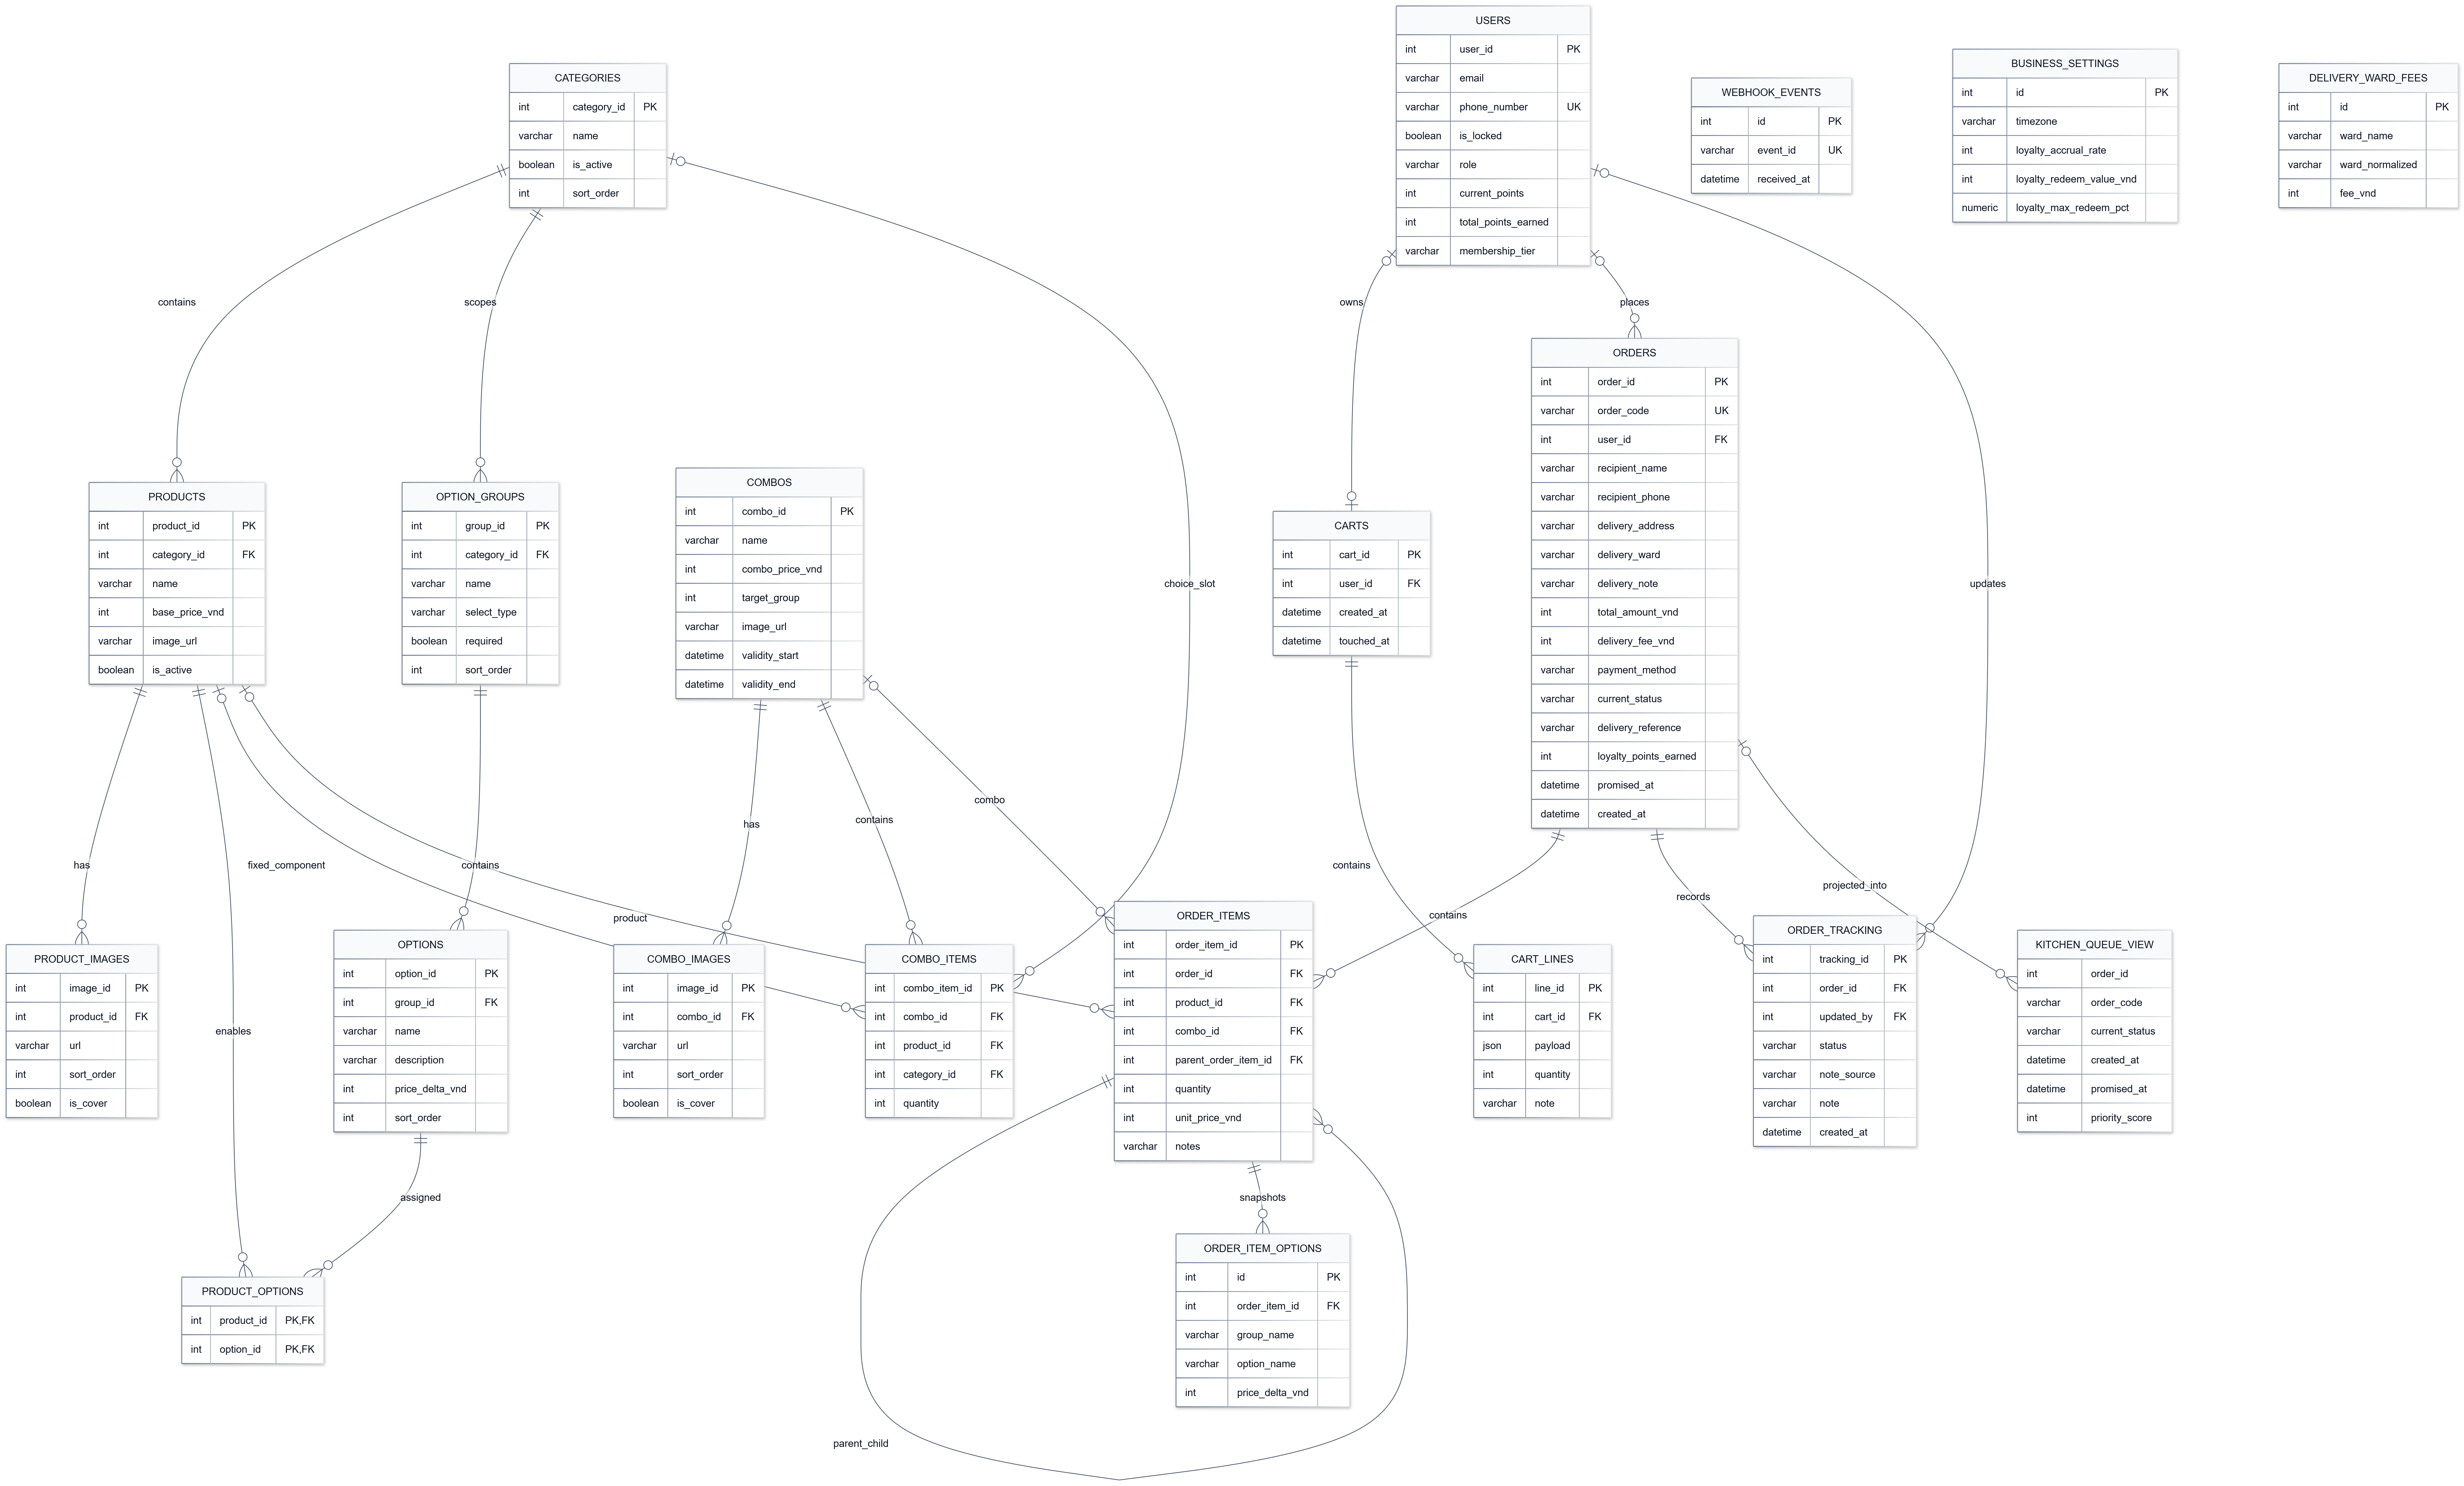
\includegraphics[width=\textwidth,height=0.84\textheight,keepaspectratio]{latex_report/figures/database_overview_full.png}
    \caption{Complete current logical ERD of PizzaHUST}
    \label{fig:database-overview-full}
\end{figure}

\begin{figure}[htbp]
    \centering
    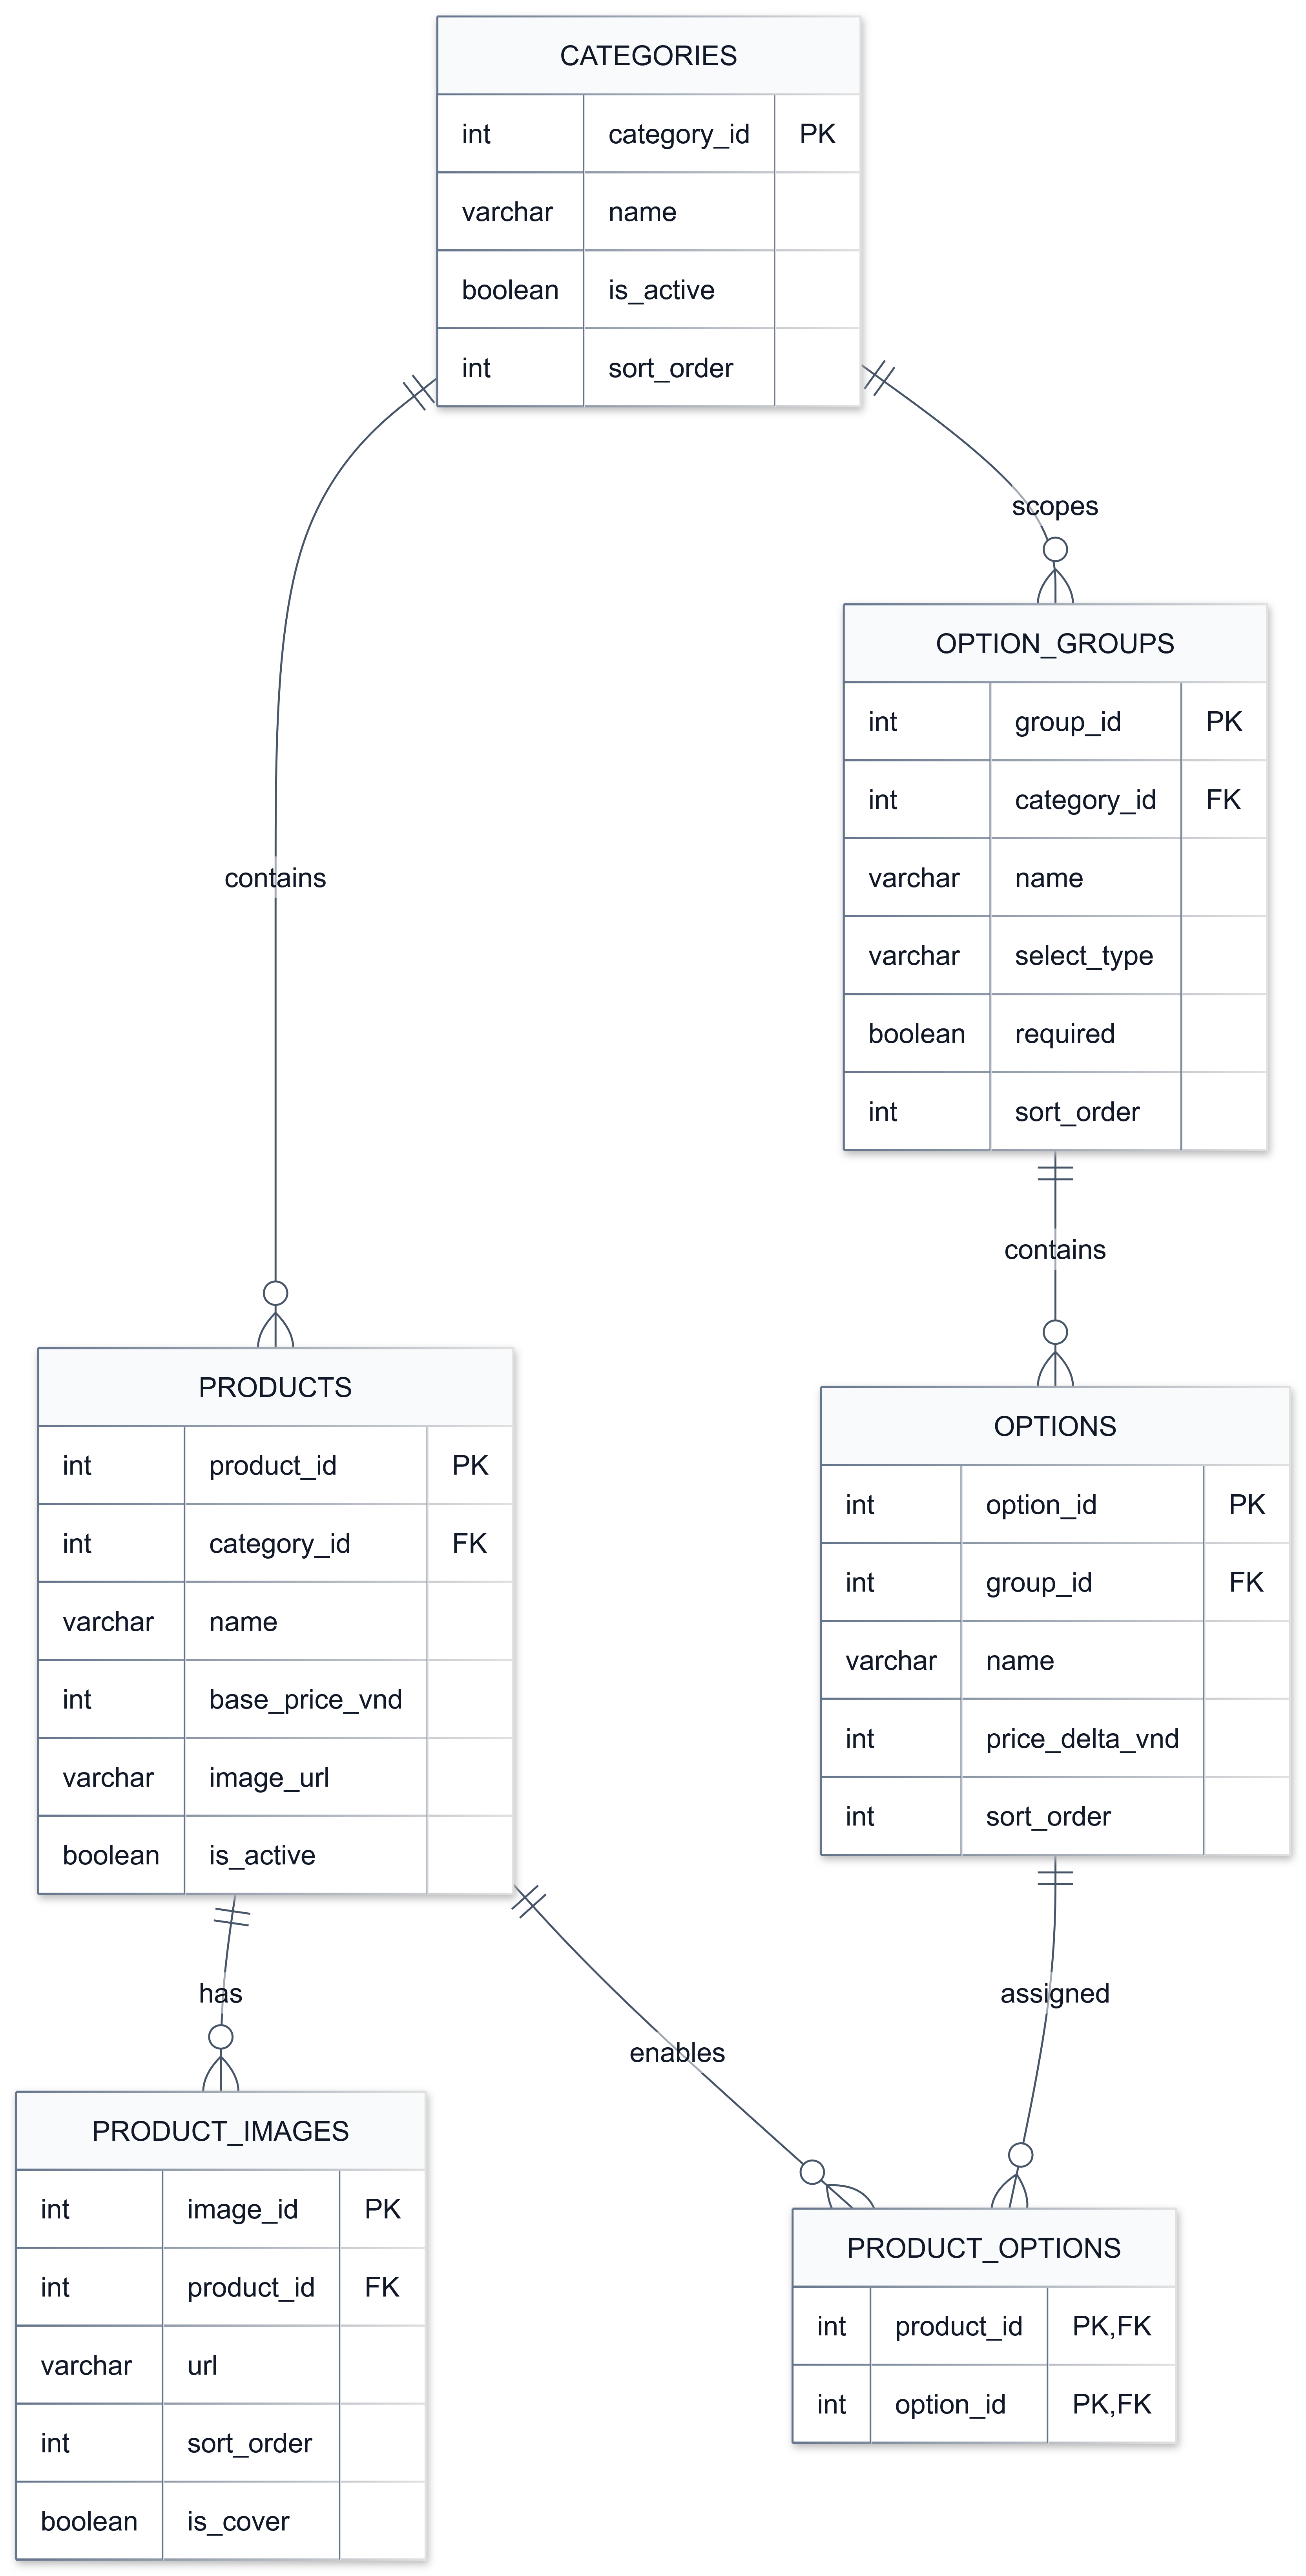
\includegraphics[width=0.86\textwidth,height=0.70\textheight,keepaspectratio]{latex_report/figures/database_catalog_options.png}
    \caption{Current catalog, image, and option-enablement relationships}
    \label{fig:database-catalog-options}
\end{figure}

\begin{figure}[htbp]
    \centering
    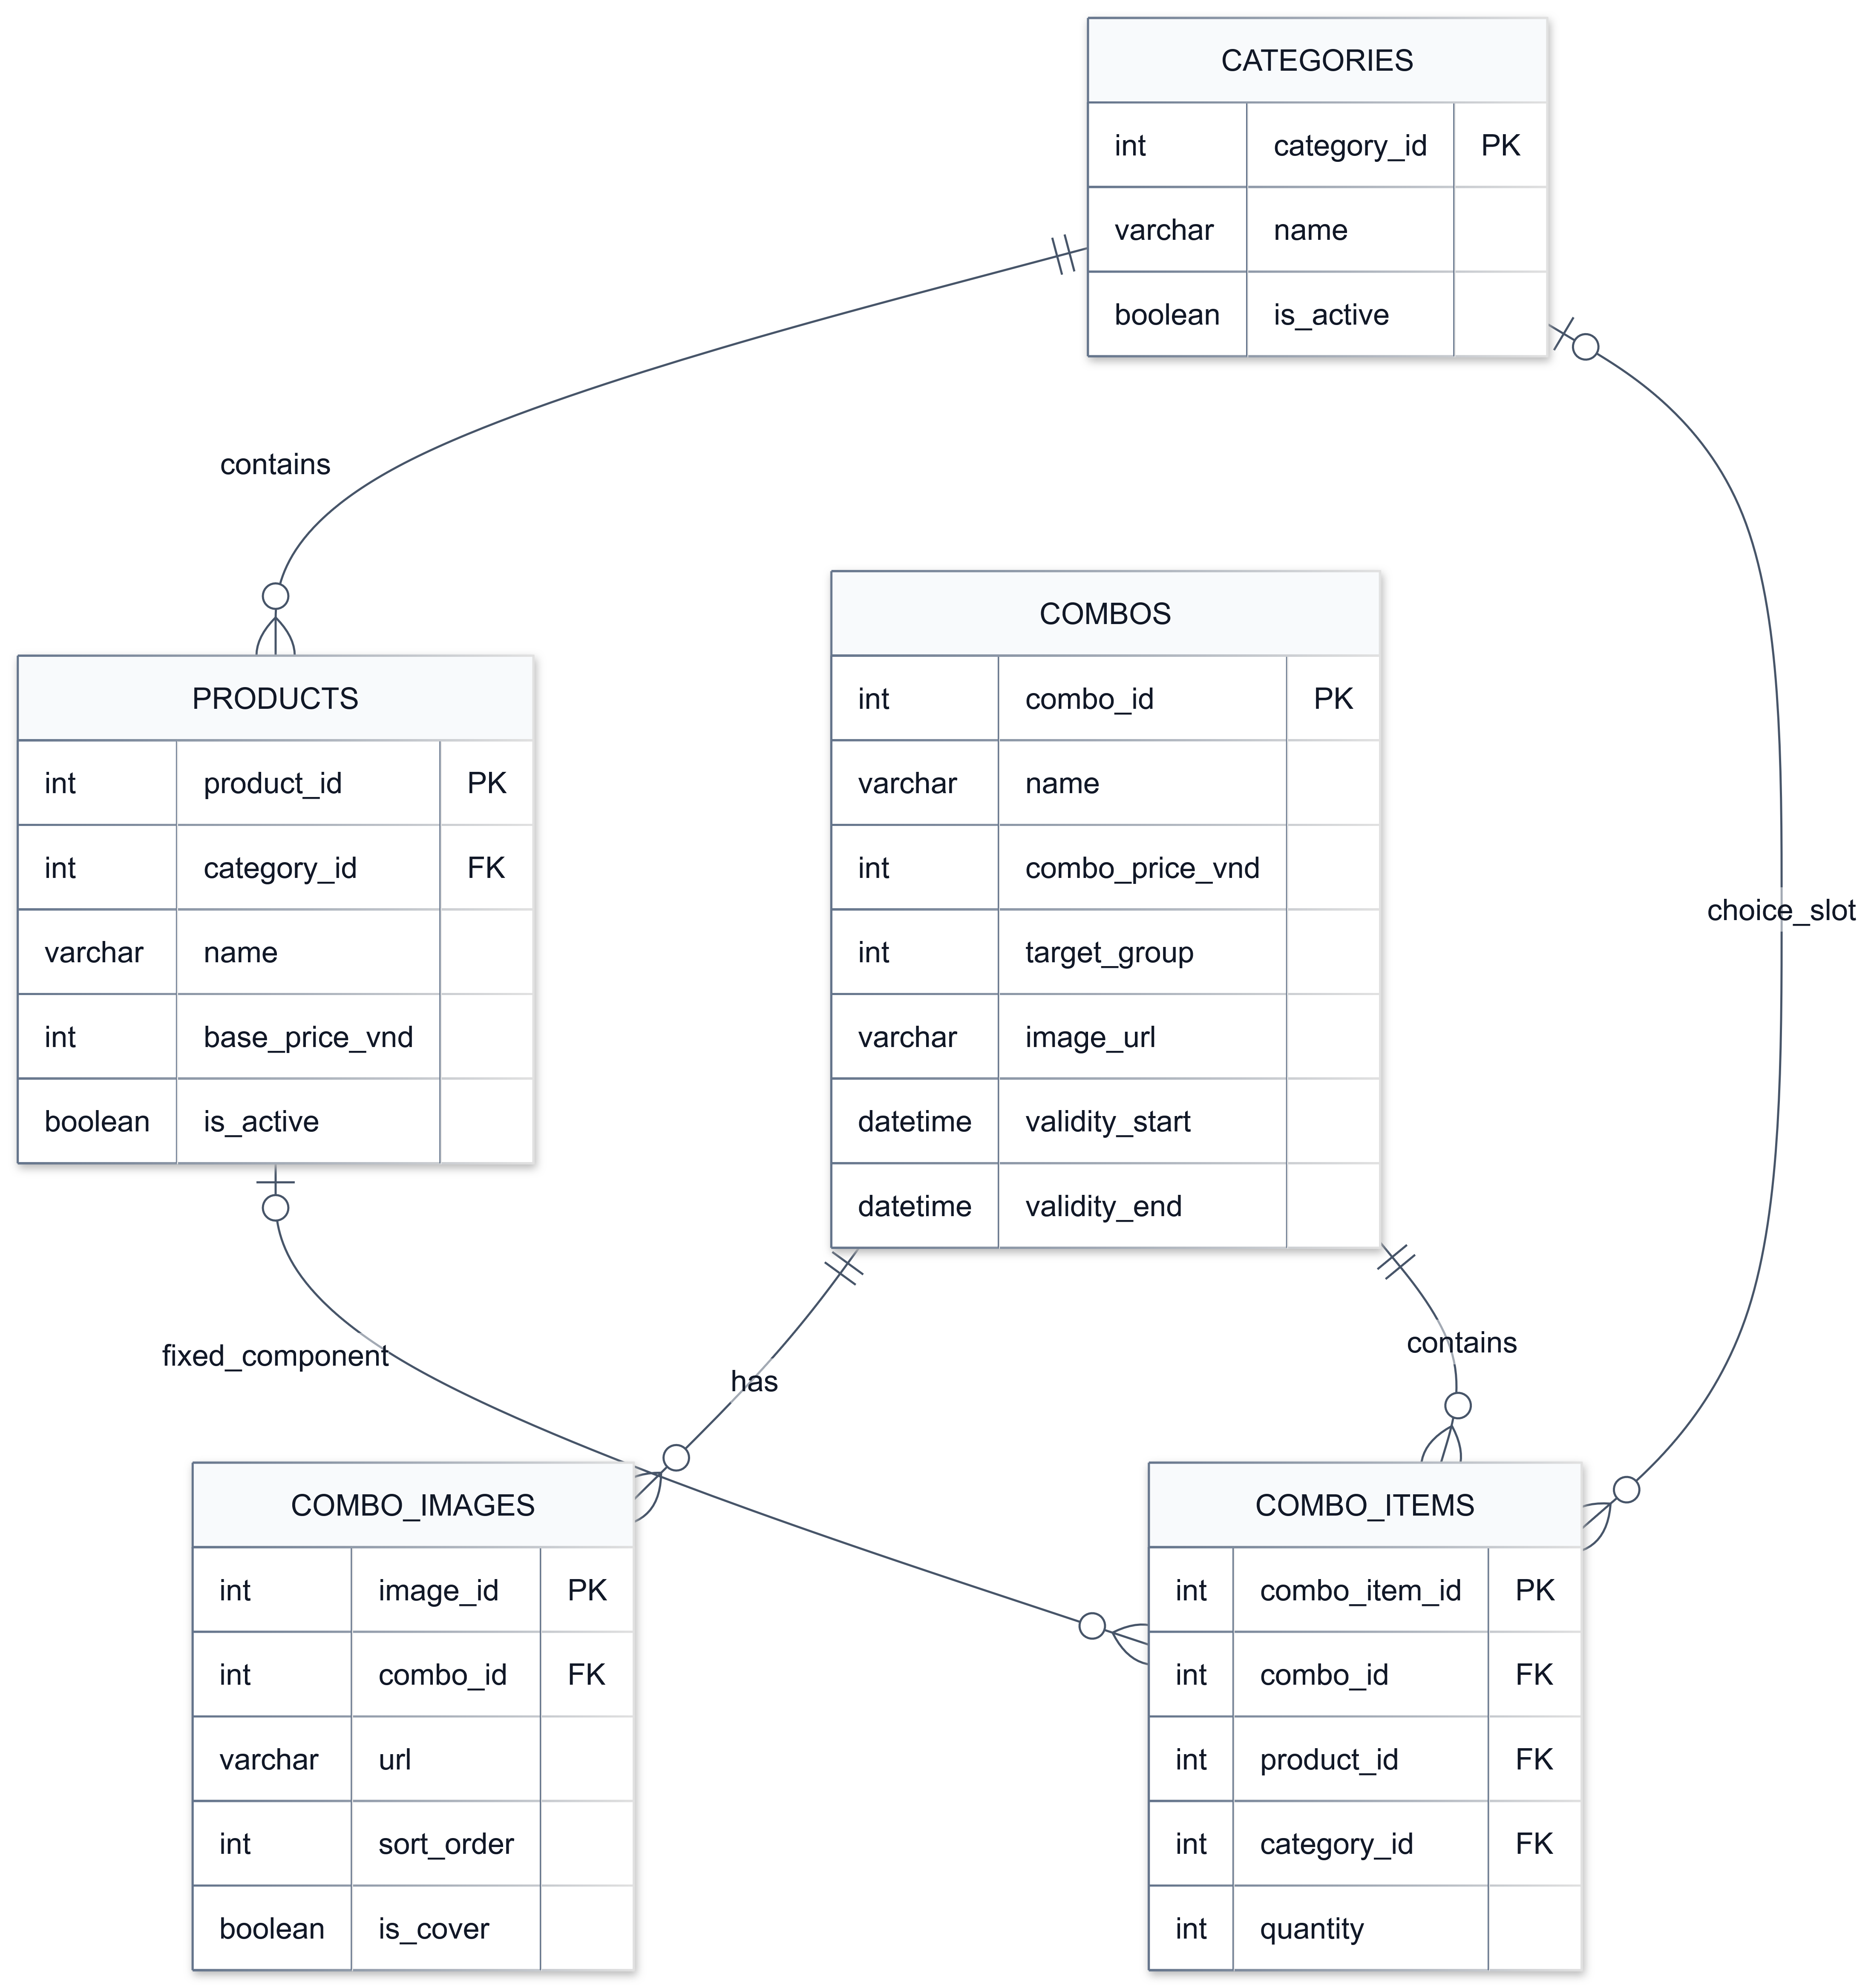
\includegraphics[width=0.86\textwidth,height=0.70\textheight,keepaspectratio]{latex_report/figures/database_combos.png}
    \caption{Current combo campaign, image, and choice-slot relationships}
    \label{fig:database-combos}
\end{figure}

\begin{figure}[htbp]
    \centering
    \includegraphics[width=0.90\textwidth,height=0.74\textheight,keepaspectratio]{latex_report/figures/database_orders.png}
    \caption{Current cart, order, tracking, and snapshot relationships}
    \label{fig:database-orders}
\end{figure}

At a high level, the most important relationships are:

\begin{itemize}
    \item each product belongs to one category;
    \item option groups are category-owned, and options belong to one option group;
    \item products enable a subset of options through the \texttt{product\_options} bridge;
    \item products and combos may each carry multiple gallery images through dedicated image tables;
    \item combos contain component rows, where each component is either a fixed product or a category-scoped choice slot;
    \item carts and cart lines preserve server-side pre-order state before order creation;
    \item orders contain multiple order items, and combo orders may decompose into parent and child order-item rows;
    \item order-item option selections are preserved as snapshots rather than live foreign-key references to mutable catalog options.
\end{itemize}

\subsection{Key integrity and business rules}

\subsubsection{Guest and registered-customer ordering}

The \texttt{orders.user\_id} reference is nullable. This allows the same order model to represent:

\begin{itemize}
    \item guest orders, which have no customer-account owner;
    \item customer orders, which are linked to a registered account.
\end{itemize}

This is a practical design because the client requires guest checkout as well as account-based features.

\subsubsection{Customization and option control}

The customization model is intentionally normalized. \texttt{option\_groups} define reusable logical groups such as sizes, crusts, or toppings, and are now scoped by category rather than treated as globally free-floating records. \texttt{options} define selectable choices and their price deltas. \texttt{product\_options} then determines which options are enabled for a given product. This avoids duplicating every option directly inside each product definition while still allowing per-product control.

\subsubsection{Combo modeling and choice slots}

Combo modeling evolved beyond a simple fixed bundle. The current schema supports an XOR-style combo component rule: a \texttt{combo\_items} row points either to a fixed \texttt{product\_id} or to a \texttt{category\_id} representing a customer's-choice slot. This is enforced through a check constraint in the current model. As a result, the database can support both rigid combos and partially customizable combo campaigns.

\subsubsection{Snapshot preservation in order history}

One of the most important database decisions is the use of \texttt{order\_item\_options} as a snapshot table. Each row stores the group name, option name, and price delta that applied at order time, without a foreign key to the live \texttt{options} table. This means administrators may later change or delete options without corrupting the historical meaning of past customer orders.

\subsubsection{Order-state and tracking history}

The order header stores the current visible lifecycle state, while \texttt{order\_tracking} stores historical state changes and related notes. This allows the application to present both the current status and a timeline of how the order reached that state. It also supports multi-actor workflow recording, since updates may originate from kitchen actions, administrative actions, system events, or transport callbacks, and the \texttt{note\_source} field records that origin explicitly.

\subsubsection{Kitchen read model}

The schema defines \texttt{kitchen\_queue\_view} as a SQL read model for queue prioritization. Rather than being a raw source-of-truth table, this object summarizes order data into a kitchen-oriented projection that can support priority-based processing behavior.

\clearpage
\section{User Interface Design}

\subsection{UI design goals}

The user interface of PizzaHUST is designed to support two very different usage contexts within one web system:

\begin{itemize}
    \item customer-facing interaction, where the priorities are discoverability, smooth ordering flow, and straightforward checkout;
    \item staff-facing operation, where the priorities are efficient management, status visibility, and operational control.
\end{itemize}

As a result, the UI design is not only about appearance. It must also express the business structure of the system clearly enough that guests, customers, administrators, and kitchen staff can each recognize the subset of the system relevant to them.

\subsection{Prototype set and design process}

The repository contains a substantial design handoff bundle in the \texttt{Design/} directory. At the time of this report, that bundle includes 28 static HTML prototype screens together with shared CSS, screenshots, and a written design brief. These prototypes are the primary source for intended visual behavior and interaction structure; they are \emph{not} production code.

The report focuses on the designed interface set represented by the mockups and the screenshots that accompany the major report use cases.

\subsection{Information architecture and navigation}

The information architecture of PizzaHUST is divided into four major navigation zones:

\begin{itemize}
    \item \textbf{Public storefront:} home, menu, item detail, combos, cart, checkout, and tracking;
    \item \textbf{Customer account area:} login, registration, account overview, and order-history-related views;
    \item \textbf{Administrative area:} items, categories, combos, customers, orders, reports, settings, and import;
    \item \textbf{Kitchen area:} queue-oriented operational view for preparing and handing off orders.
\end{itemize}

Public-facing routes use shared site chrome with top navigation, footer, theme control, and account/cart entry points. Administrative routes switch to a more tool-oriented layout with a dedicated side navigation structure. Kitchen-facing routes emphasize queue clarity and action availability rather than marketing or browsing concerns.

The screenshot set below documents the UI for the core report scope. By request, the integration-only T1/T2 flow is excluded from the UI section because it does not have a dedicated user-facing screen.

\newcommand{\uifig}[3]{%
\begin{figure}[htbp]
    \centering
    \includegraphics[width=0.94\textwidth,height=0.62\textheight,keepaspectratio]{\detokenize{latex_report/UI Design/#1}}
    \caption{#2}
    \label{#3}
\end{figure}
}

\subsection{Customer storefront screens}

\uifig{Menu_U1.png}{Customer menu discovery screen for U1 Browse Menus}{fig:ui-u1-menu}
\uifig{Item_Detail_U2.png}{Customer item detail screen for U2 View Item Details}{fig:ui-u2-item-detail}
\uifig{Customize_Pizza_U3.png}{Pizza customization screen for U3 Customize Pizza}{fig:ui-u3-customize-pizza}
\uifig{Combos_U4.png}{Combo promotion listing for U4 View Combo Promotions}{fig:ui-u4-combos}
\uifig{Combos_Details_U4.1.png}{Combo detail and slot customization screen for U15 Customize Combo}{fig:ui-u15-combo-detail}
\uifig{Cart_U5.png}{Shopping cart screen for U5 Manage Cart}{fig:ui-u5-cart}
\uifig{Place_COD_U6.png}{Checkout screen for U6 Place COD Order}{fig:ui-u6-checkout}
\uifig{Track_Order_U7.png}{Order tracking screen for U7 Track Order}{fig:ui-u7-track}
\FloatBarrier

\subsection{Customer account screens}

\uifig{Register_U8.png}{Registration form for U8 Register}{fig:ui-u8-register}
\uifig{Log_In_U9.png}{Login form for U9 Log In}{fig:ui-u9-login}
\uifig{Order_History_U11.png}{Order history screen for U11 View Order History}{fig:ui-u11-order-history}
\uifig{Manage_Profile_U12.png}{Profile management screen for U12 Manage Profile}{fig:ui-u12-profile}
\uifig{Loyalty_Point_U13.png}{Loyalty balance and activity screen for U13 View Loyalty Points}{fig:ui-u13-loyalty}
\uifig{Redeem_Loyalty_point_U14.png}{Checkout loyalty redemption screen for U14 Redeem Points for Discount}{fig:ui-u14-redeem}
\FloatBarrier

\subsection{Administrative screens}

\uifig{Pizza_Catalog_A1.png}{Pizza catalog management screen for A1 Manage Pizza Catalog}{fig:ui-a1-catalog}
\uifig{A2_Manage_Pizza_Option.png}{Pizza option management screen for A2 Manage Pizza Options and Side Dishes}{fig:ui-a2-options}
\uifig{A2_Manage_Side_Dishes.png}{Side-dish management screen for A2 Manage Pizza Options and Side Dishes}{fig:ui-a2-sides}
\uifig{A3_Menu_Categories_Overview.png}{Category management overview for A3 Manage Menu Categories}{fig:ui-a3-categories-overview}
\uifig{A3_Menu_Categories_Detailed.png}{Category management detail for A3 Manage Menu Categories}{fig:ui-a3-categories-detail}
\uifig{A4_Combo_Campain_Overview.png}{Combo campaign overview for A4 Manage Combo Campaigns}{fig:ui-a4-combos-overview}
\uifig{A4_Combo_Campain_Detailed.png}{Combo campaign detail for A4 Manage Combo Campaigns}{fig:ui-a4-combos-detail}
\uifig{A5_Order_Delivery_monitor.png}{Order and delivery monitoring screen for A5 Monitor Orders and Delivery Exceptions}{fig:ui-a5-orders}
\uifig{A6_Customer_Acc_Management.png}{Customer account management screen for A6 Manage Customer Accounts}{fig:ui-a6-customers}
\uifig{A7_Sale_Order_Report.png}{Sales and order reporting screen for A7 View Sales and Order Reports}{fig:ui-a7-reports}
\FloatBarrier

\subsection{Kitchen screens}

\uifig{K1_Incoming_Orders.png}{Kitchen queue screen for K1 View Incoming Orders}{fig:ui-k1-queue}
\uifig{K2_Accept_Order.png}{Kitchen accept-order action screen for K2 Update Preparation Status}{fig:ui-k2-accept}
\uifig{K3_Mark_Ready_For_Dispatch.png}{Kitchen mark-ready screen for K3 Mark Order Ready for Dispatch}{fig:ui-k3-ready}
\FloatBarrier

\subsection{Visual system}

The design language of PizzaHUST combines an ordering-oriented storefront aesthetic with more functional operational layouts for staff views. The production frontend currently uses:

\begin{itemize}
    \item local Poppins font assets for consistent typography;
    \item token-based light and dark themes;
    \item reusable navigation and content shells;
    \item card-based presentation for menu, combo, and administrative summary surfaces;
    \item action-oriented controls for kitchen and admin workflows.
\end{itemize}

The storefront is optimized around browsing, visual comparison, and ordering progression, while the administrative and kitchen interfaces prioritize table/list clarity, status visibility, and action placement. This difference is important because a single design language would not serve all actor groups equally well.

\subsection{Responsive behavior and accessibility considerations}

PizzaHUST is explicitly designed as a responsive web application rather than a desktop-only staff tool or a mobile-only consumer app. The production code uses responsive Tailwind utility classes to adapt page layout and interaction density across viewport sizes.

The current codebase also shows accessibility intent in several areas:

\begin{itemize}
    \item labels and accessible naming for controls;
    \item focus visibility and state indication;
    \item \texttt{aria-live} usage for dynamic feedback in quote or quantity-related interactions;
    \item semantic selection behavior such as radio-style option controls and pressed-state indicators;
    \item accessible mobile navigation handling.
\end{itemize}

However, the report should state clearly that no formal accessibility audit artifact was found in the repository. The interface should therefore be described as having \emph{accessibility-aware implementation intent}, not as a fully audited accessible product.

\clearpage
\section{Component Implementation}

\subsection{Implementation strategy}

PizzaHUST has been implemented as a set of vertical slices that connect frontend routes, backend APIs, domain rules, persistence structures, and verification artifacts. This is a more meaningful way to present implementation than listing files in isolation, because the system's value comes from complete workflows rather than from disconnected modules.

At the same time, the implementation section must remain grounded in the current repository state. The report therefore focuses on the strongest implemented slices first and describes the complete system coverage as it exists now.

\subsection{Implemented vertical slices}

\begingroup
\footnotesize
\setlength{\LTpre}{0.4em}
\setlength{\LTpost}{0.8em}
\captionof{table}{Current implementation vertical slices}\label{tab:application-slices}
\begin{tabular}{L{0.15\linewidth} L{0.22\linewidth} L{0.27\linewidth} L{0.26\linewidth}}
\toprule
\textbf{Vertical slice} & \textbf{Frontend entry points} & \textbf{Backend and domain focus} & \textbf{Persistence / verification anchor} \\
\midrule
Public catalog & Home, menu, item pages & category and item APIs, read models & products/categories schema, menu tests \\
Pizza customization and quote & Item detail customizer & cart quote API, pricing domain, option validation & option tables, pricing/quote tests \\
Combo browsing and customization & Combo list and combo detail pages & combo APIs, combo-slot rules, surcharge logic & combos/combo\_items schema, combo tests \\
Cart and order placement & Cart, checkout, order confirmation & cart state, order creation, order-code generation & carts/orders/order\_items schema, checkout/order tests \\
Authentication and session flow & Login, register, account surfaces & auth routes, password hashing, session state, CSRF & user model, auth tests \\
Administrative catalog & Admin items, categories, combos, import & admin CRUD routers, validation logic & catalog migrations, admin tests \\
Administrative operations & Admin orders, customers, reports, settings & operational APIs, customer controls, reporting logic & order/user/reporting persistence, admin ops tests \\
Kitchen and delivery coordination & Kitchen page, tracking-related progression & kitchen actions, delivery port, webhook sync & order tracking, webhook events, kitchen/delivery tests \\
\bottomrule
\end{tabular}
\endgroup

\subsection{Representative business-rule implementation}

\subsubsection{Server-authoritative pricing}

Pricing is intentionally implemented on the backend rather than in the browser. The quotation pipeline resolves the selected item or combo structure against current database state, validates the chosen options, applies combo discount logic, adds delivery-fee rules where appropriate, and computes the final total in integer VND. This approach prevents pricing drift between UI logic and business logic and makes the quote path testable at backend level.

\subsubsection{Generic option validation}

The generic options model is one of the clearest examples of reusable business logic. Option groups can be single-select or multi-select and may also be required. Validation ensures that selected options are actually enabled for the product, that required groups are satisfied, and that single-select groups do not contain conflicting choices. This logic is reused both for direct product ordering and for product picks nested inside combos.

\subsubsection{Combo choice-slot handling}

Combo implementation goes beyond static bundle storage. When a combo contains a category-scoped slot, the implementation determines the reference product price for that category and calculates a surcharge only when the selected product exceeds that reference baseline. This allows customizable combos while preserving deterministic pricing logic.

\subsubsection{Order-state transitions}

The order-state implementation is centralized in the domain layer. Only explicitly allowed transitions are valid, including cancellation, courier-handoff fallback, delivery completion, and delivery failure. By concentrating this logic in one place, the system avoids duplicating state-machine rules across admin actions, kitchen actions, and webhook processing.

\subsection{Integration implementation}

\subsubsection{Delivery-port abstraction}

Delivery integration is implemented through a provider-neutral port abstraction. The business workflow does not call raw HTTP directly from every order-related action; instead, delivery requests are routed through a delivery interface and adapter layer. This keeps the ordering workflow cleaner and makes it possible to substitute mock and real provider implementations.

\subsubsection{Mock-first delivery workflow}

The current repository uses a dedicated delivery-mock service as the practical integration target for development and verification. The mock accepts dispatch requests, stores lightweight job state, advances through delivery events, and sends signed callbacks back to the main backend. This gives the project a realistic integration path even without depending on a live commercial courier API.

\subsubsection{Operational fallback behavior}

The implementation also includes operational fallback logic. If the normal dispatch path fails or if pickup confirmation from the courier side does not arrive as expected, the system can preserve consistency through exception states or manual continuation paths rather than silently leaving the order in an ambiguous condition. This is a strong implementation choice for a workflow-heavy application.

\subsection{Implementation coverage}

The current repository demonstrates strong implementation coverage across:

\begin{itemize}
    \item menu browsing and item detail;
    \item pizza customization and authoritative quotation;
    \item combo browsing and core combo customization behavior;
    \item cart handling and COD order placement;
    \item authentication infrastructure;
    \item administrative catalog management;
    \item administrative operational views;
    \item kitchen state actions and delivery callback synchronization.
\end{itemize}

\clearpage
\section{API Design and Implementation}

\subsection{API style and conventions}

PizzaHUST exposes a REST-style HTTP API under the \texttt{/api} namespace. The backend publishes an OpenAPI description at \texttt{/api/openapi.json}, and the current frontend uses generated TypeScript types derived from that contract. JSON is the default data format for request and response bodies, while multipart upload is reserved for specific cases such as image uploads and CSV import.

Several contract conventions are used consistently:

\begin{itemize}
    \item money values are represented as integer VND amounts;
    \item timestamps use ISO 8601 date-time formatting;
    \item internal database-backed resources use integer identifiers;
    \item public guest order tracking uses an order code rather than exposing internal IDs.
\end{itemize}

These conventions reduce ambiguity across the frontend, backend, and testing layers.

\subsection{Authentication and security model}

The API is designed for a browser-based session workflow rather than token-only SPA authentication. Authenticated access depends on a signed session cookie managed by the backend. The frontend API client sends requests with browser credentials enabled and automatically attaches a CSRF token header for mutating requests when the token is present in cookies.

Role-restricted actions are enforced in the backend through dependency-based guards. This means the same API host can expose:

\begin{itemize}
    \item public routes for browsing, quoting, and some guest-facing order functions;
    \item customer-only routes for account and loyalty behavior;
    \item admin-only routes for catalog, order, customer, settings, and reporting management;
    \item kitchen-only routes for operational queue actions;
    \item externally callable webhook routes protected by message authentication.
\end{itemize}

\subsection{Error model}

PizzaHUST does not return arbitrary error shapes. Non-success responses are normalized into an error envelope containing:

\begin{itemize}
    \item an application-level error code;
    \item a human-readable message;
    \item optional structured details;
    \item the current request ID.
\end{itemize}

This is important for two reasons. First, frontend code can respond consistently to expected failures such as validation errors, unauthorized access, or business-state conflicts. Second, the request ID allows debugging and log correlation across the backend boundary.

The current backend error handling maps raw HTTP failures into a closed contract-level code set, including validation, authentication, authorization, conflict, rate limiting, and delivery-upstream errors.

\subsection{API surface by module}

The current OpenAPI file contains 63 documented paths. Table~\ref{tab:api-surface} groups them by functional area.

\begingroup
\small
\setlength{\LTpre}{0.4em}
\setlength{\LTpost}{0.8em}
\captionof{table}{Current API surface grouped by module}\label{tab:api-surface}
\begin{tabular}{L{0.19\linewidth} L{0.10\linewidth} L{0.18\linewidth} L{0.43\linewidth}}
\toprule
\textbf{API group} & \textbf{Paths} & \textbf{Typical access} & \textbf{Main purpose} \\
\midrule
Health & 1 & Public & Service health check for runtime readiness. \\
Configuration & 3 & Public & Read delivery, loyalty, and business-setting values needed by the frontend. \\
Catalog & 3 & Public & Browse categories and item list/detail data. \\
Combos & 2 & Public & Browse combo list and combo detail data. \\
Cart & 5 & Public or session-backed & Quote, retrieve, and manage cart state. \\
Orders & 5 & Mixed & Place orders, track orders, and retrieve customer order history. \\
Authentication & 4 & Mixed & Register, login, logout, and inspect/update current account state. \\
Loyalty & 1 & Customer session & Return loyalty summary data. \\
Administrator & 33 & \texttt{admin} role & Manage catalog, options, combos, customers, orders, reports, import, and settings. \\
Kitchen & 5 & \texttt{kitchen} role & View operational order data and perform kitchen-side actions. \\
Webhooks & 1 & HMAC protected & Accept external delivery-status callbacks. \\
\bottomrule
\end{tabular}
\endgroup

This grouping shows that the administrative surface is the largest part of the API. That is consistent with the system's dual nature as both a customer storefront and a store-operation platform.

\subsection{Representative endpoint behavior}

Representative endpoints are more useful than a raw endpoint list because they illustrate how the API applies validation, authorization, and business rules in practice.

\begingroup
\small
\setlength{\LTpre}{0.4em}
\setlength{\LTpost}{0.8em}
\captionof{table}{Representative endpoint behavior}\label{tab:representative-endpoints}
\begin{tabular}{L{0.20\linewidth} L{0.32\linewidth} L{0.39\linewidth}}
\toprule
\textbf{Method and path} & \textbf{Purpose} & \textbf{Important behavior} \\
\midrule
\texttt{GET /api/items/\{id\}} & Return one active menu item. & Returns item details and enabled option groups for customer-side customization; inactive items are not treated as valid public resources. \\
\texttt{POST /api/cart/quote} & Compute an authoritative preview quote. & Deduplicates selected option IDs, validates option rules and combo selections, resolves live prices from the database, and optionally checks delivery-area rules. \\
\texttt{POST /api/orders} & Place a COD order from cart state. & Converts validated cart lines into a durable order, creates an order code, persists item snapshots, and rejects invalid cart or address state. \\
\texttt{POST /api/auth/login} & Start an authenticated customer/admin/kitchen session. & Validates credentials, enforces account restrictions, sets session and CSRF cookies, and uses controlled error handling for authentication failure. \\
\texttt{POST /api/admin/orders/\{id\}/retry-dispatch} & Retry delivery handoff for an exception order. & Requires administrative access, permits only valid retry states, and preserves consistency if the upstream delivery provider fails again. \\
\texttt{POST /api/kitchen/orders/\{id\}/mark-ready} & Move a prepared order toward dispatch. & Enforces kitchen authorization, validates workflow state, and may produce either \texttt{ReadyForDispatch} or a retryable handoff-failure state depending on delivery-port outcome. \\
\texttt{POST /api/webhooks/delivery} & Accept courier status synchronization. & Requires HMAC validation, uses idempotency protection, maps provider states into internal order-state rules, and records tracking updates only for valid transitions. \\
\bottomrule
\end{tabular}
\endgroup

\subsection{Representative request/response patterns}

The design of the API can also be seen in the structure of a few core request/response patterns:

\begin{itemize}
    \item \textbf{Quote requests} accept candidate cart lines and optional address information, but never trust the client to supply price values.
    \item \textbf{Order placement requests} collect delivery information and optional notes, then transform session-backed cart state into durable business records.
    \item \textbf{Administrative mutation requests} rely on session role checks plus CSRF protection, reflecting the browser-based staff UI model.
    \item \textbf{Webhook requests} invert the normal user-driven pattern by accepting externally initiated state changes under strict signature validation.
\end{itemize}

These patterns show that the API is designed around business workflows rather than only CRUD-style resource manipulation.

\subsection{Contract generation and drift control}

Contract discipline is one of the strongest technical aspects of the current PizzaHUST implementation. The backend exports the OpenAPI document automatically, and the project verification pipeline checks that the committed contract file remains synchronized with generated output. The frontend then regenerates \texttt{lib/api/types.ts} from the OpenAPI description and checks that the generated type file has not drifted.

This workflow provides two important benefits:

\begin{itemize}
    \item it reduces the risk that frontend request/response assumptions silently diverge from backend behavior;
    \item it turns the API specification into a maintained artifact rather than a document that becomes stale after implementation changes.
\end{itemize}

\subsection{Interaction-flow diagrams}

The existing sequence diagrams are still useful as high-level illustrations of the main order-processing interactions. They show the coordination between browsing, quotation, checkout, kitchen progression, delivery handoff, and tracking, not just isolated endpoint calls.

\begin{figure}[htbp]
    \centering
    
\includegraphics[page=2,width=0.92\textwidth,height=0.68\textheight,keepaspectratio]{latex_report/figures/order_flow_implemented.pdf}
    \caption{Implemented quotation-focused API interaction flow}
    \label{fig:order-flow-quotation}
\end{figure}

\begin{figure}[htbp]
    \centering
    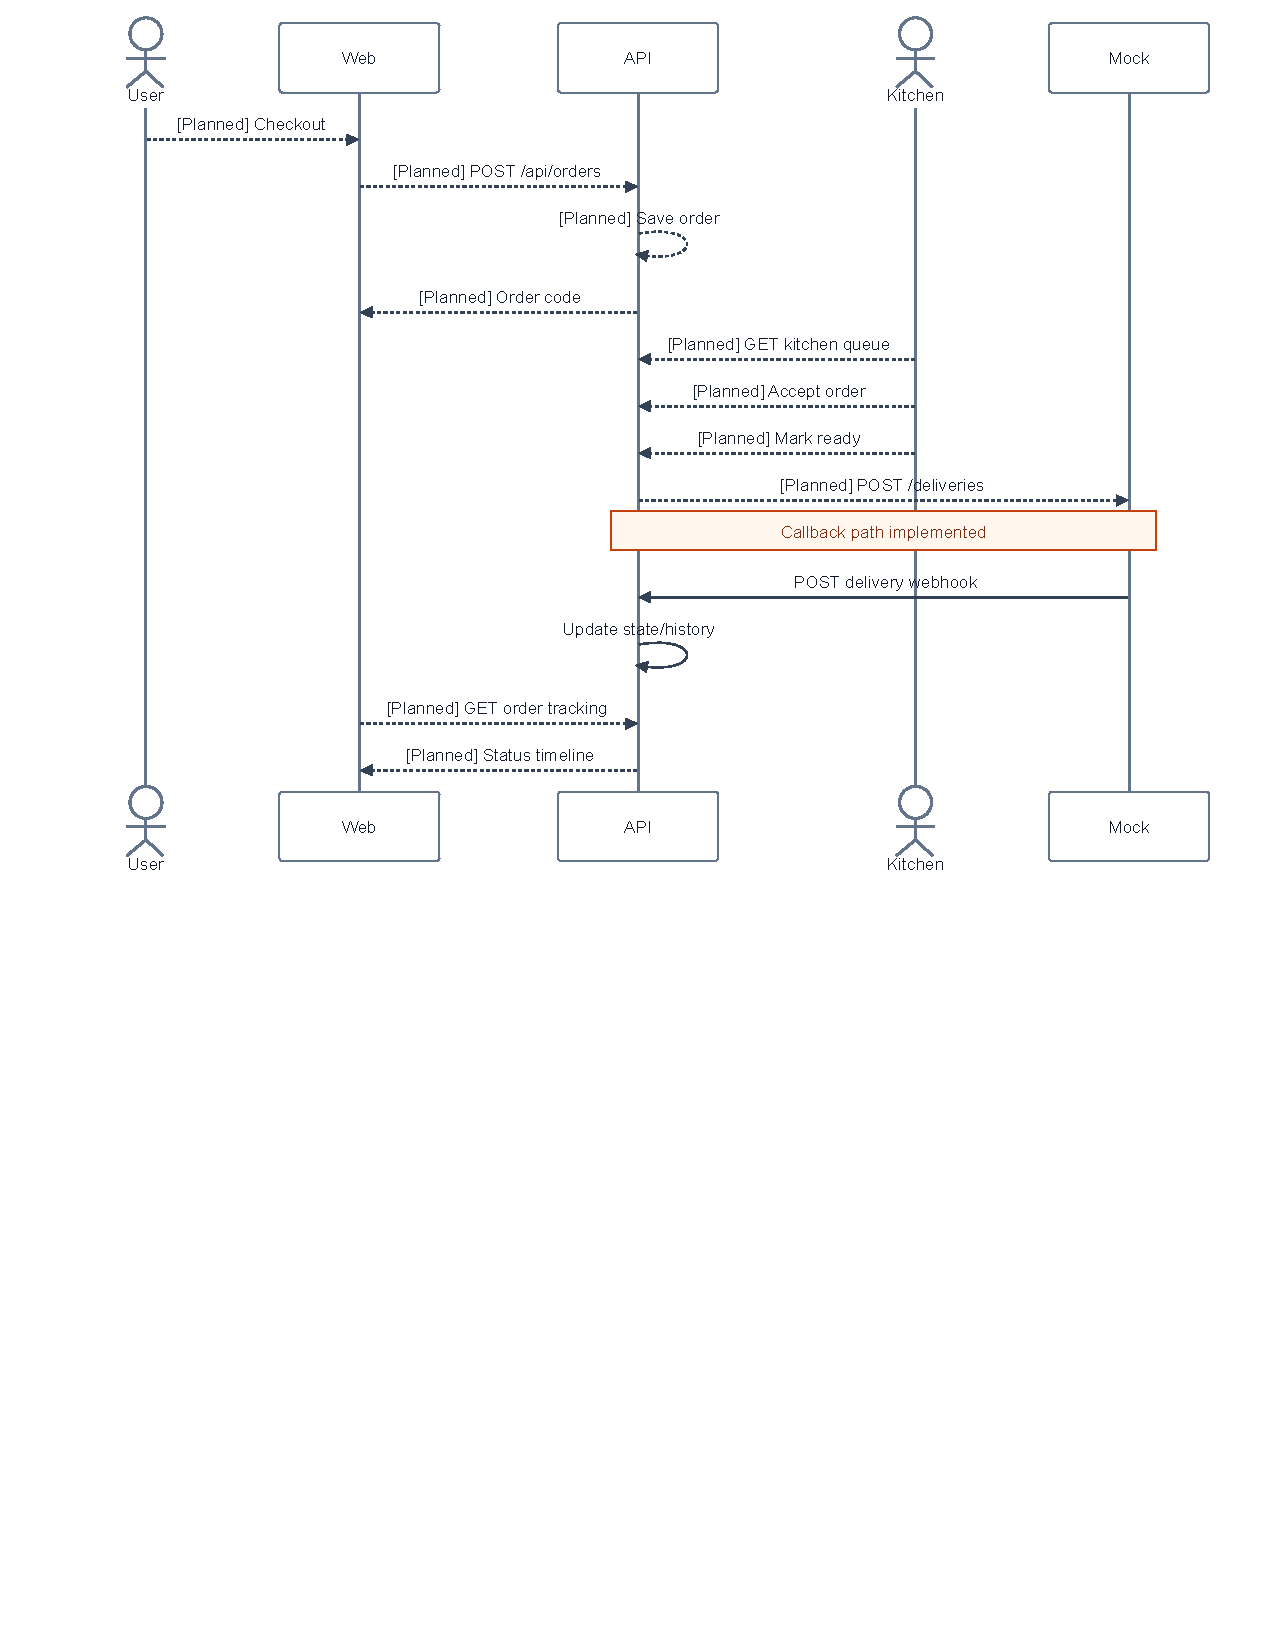
\includegraphics[width=\textwidth,height=0.78\textheight,keepaspectratio,trim=55 368 25 5,clip]{latex_report/figures/order_flow_delivery_flow.pdf}
    \caption{Broader order-processing and delivery-tracking interaction flow}
    \label{fig:order-flow-delivery-tracking}
\end{figure}

The first diagram aligns more directly with already implemented quotation behavior, while the second represents the broader end-to-end workflow view.

\subsection{API coverage}

This API section describes the current implementation and the full contract surface. The repository contains substantial operational endpoints for catalog browsing, pricing, order placement, administrative management, kitchen actions, customer-account features, loyalty, and delivery synchronization. The report therefore presents the API as a strong, structured contract surface that is now aligned with the completed product scope.

\clearpage
\section{Testing and Evaluation}

\subsection{Test strategy}

PizzaHUST uses a layered testing and verification strategy rather than relying on a single test style. This is appropriate because the project includes:

\begin{itemize}
    \item business-rule-heavy backend logic;
    \item a browser-based frontend with staff and customer views;
    \item schema evolution through migrations;
    \item generated API contracts;
    \item a realistic external integration boundary through the delivery mock.
\end{itemize}

As a result, quality assurance is distributed across static checks, backend tests, frontend unit tests, browser tests, schema and contract drift checks, and smoke-style end-to-end verification.

\begingroup
\small
\setlength{\LTpre}{0.4em}
\setlength{\LTpost}{0.8em}
\captionof{table}{Testing and quality-assurance layers}\label{tab:test-artifacts}
\begin{tabular}{L{0.20\linewidth} L{0.34\linewidth} L{0.38\linewidth}}
\toprule
\textbf{Layer} & \textbf{Tool or mechanism} & \textbf{Main purpose} \\
\midrule
Static backend quality & Ruff, Ruff format, mypy, import-linter & Enforce code quality, type discipline, and boundary rules. \\
Backend unit and integration tests & pytest and httpx-based tests & Verify domain logic, API behavior, persistence rules, and integration behavior. \\
Schema and contract drift checks & Alembic check and OpenAPI comparison & Detect mismatch between code, schema, and published API contract. \\
Static frontend quality & TypeScript, ESLint, Next.js build & Protect type correctness, lint quality, and production buildability. \\
Frontend unit tests & Vitest & Verify helper functions, API wrappers, component logic, and selected route behavior. \\
Browser workflow tests & Playwright & Validate important user-facing paths through real browser interaction. \\
Smoke end-to-end verification & Compose + pytest smoke flow & Validate the intended cross-service business flow in a realistic local runtime stack. \\
\bottomrule
\end{tabular}
\endgroup

\subsection{Verification workflow}

The strongest testing artifact in the repository is the verification script \texttt{Application/verify.sh}. It acts as the practical definition-of-done gate by executing the quality layers in a fixed sequence:

\begin{enumerate}
    \item backend linting and formatting checks;
    \item backend type and import-boundary checks;
    \item backend test suite;
    \item migration drift verification;
    \item OpenAPI export and drift comparison;
    \item frontend type generation and drift verification;
    \item frontend linting, unit tests, and production build;
    \item smoke-style backend end-to-end test flow;
    \item Playwright browser workflow tests.
\end{enumerate}

This workflow is valuable because it ties source quality, contract accuracy, schema consistency, and browser-facing behavior into one repeatable verification pipeline rather than treating them as separate ad hoc checks.

\subsection{Current test inventory}

At the time of this report revision, the repository contains the following visible test inventory:

\begin{itemize}
    \item 60 backend test files matching \texttt{test\_*.py};
    \item 24 frontend unit/component test files matching \texttt{*.test.ts} or \texttt{*.test.tsx};
    \item 24 Playwright browser specification files matching \texttt{*.spec.ts};
    \item 29 route-page files in the frontend application;
    \item 63 documented API paths in the current OpenAPI contract.
\end{itemize}

These counts are useful as scale indicators, although they do not by themselves prove quality. The more important point is the spread of verification across major functional areas.

\subsection{Representative subsystem coverage}

\subsubsection{Backend domain and API coverage}

The backend tests cover major business-rule areas such as:

\begin{itemize}
    \item pricing and quote logic;
    \item option validation;
    \item combo and combo-slot behavior;
    \item authentication and security-related behavior;
    \item catalog and administrative operations;
    \item delivery adapter and webhook handling;
    \item order-state transitions;
    \item reporting and settings behavior.
\end{itemize}

This is especially important because much of PizzaHUST's correctness depends on domain behavior rather than only on surface rendering.

\subsubsection{Frontend and browser coverage}

Frontend unit tests and Playwright tests cover a broad range of user-visible behavior, including:

\begin{itemize}
    \item menu browsing and item detail flows;
    \item cart and checkout;
    \item login and registration;
    \item combo customization;
    \item tracking;
    \item administrator catalog and operations pages;
    \item kitchen-facing UI behavior;
    \item theme and selected shared UI logic.
\end{itemize}

This gives the project meaningful verification at both the logic-helper level and the browser-workflow level.

\subsubsection{Integration and workflow coverage}

The smoke and integration layers are important because PizzaHUST is not just a collection of isolated pages. Order placement, kitchen progression, dispatch handoff, and delivery synchronization are cross-component workflows. The inclusion of delivery-mock integration, webhook handling, and smoke-style end-to-end flows significantly improves confidence in the operational parts of the system.

\subsection{Evaluation against project goals}

\begingroup
\small
\setlength{\LTpre}{0.4em}
\setlength{\LTpost}{0.8em}
\captionof{table}{Evaluation of the current implementation and verification approach}\label{tab:project-evaluation}
\begin{tabular}{L{0.23\linewidth} L{0.70\linewidth}}
\toprule
\textbf{Evaluation area} & \textbf{Assessment} \\
\midrule
Functional correctness & Strongest in catalog browsing, customization, cart/ordering, administrative operations, and delivery-related workflows due to combined backend, frontend, and browser coverage. \\
Architecture quality & Supported by import-boundary enforcement, contract generation, migration checks, and the modular monolith structure. \\
Reliability & Strengthened by explicit order-state rules, delivery idempotency, exception-handling paths, and smoke-style workflow verification. \\
Security & Supported by session authentication, role guards, CSRF handling, rate limiting, and HMAC-protected webhook processing. \\
Maintainability & Improved by layered backend structure, generated API types, migration history, and centralized verification workflow. \\
Usability confidence & Supported by responsive implementation and browser tests, though not by a formal UX study. \\
Deployment confidence & Supported at local/demo level through Compose and verification automation, with clear workflow coverage and repeatable checks. \\
\bottomrule
\end{tabular}
\endgroup

\subsection{Limitations and remaining risks}

The testing and evaluation section must also state the current evaluation boundaries clearly:

\begin{itemize}
    \item no formal accessibility audit report was found in the repository;
    \item no production-scale performance benchmark was found;
    \item local Compose-based verification is strong evidence for development readiness, but it is not the same as long-term production validation.
\end{itemize}

These limitations do not negate the quality of the project, but they define the boundary of what the report can honestly claim.

\subsection{Overall evaluation}

PizzaHUST demonstrates substantial software-engineering value across requirements refinement, UI prototyping, modular implementation, schema evolution, contract discipline, and workflow-heavy backend logic. Its most convincing technical strengths are:

\begin{itemize}
    \item authoritative backend pricing and validation;
    \item strong admin/catalog operational support;
    \item explicit order-state workflow control;
    \item realistic mock-first external integration;
    \item a verification pipeline that combines static quality, contract checks, backend tests, frontend tests, and browser flows.
\end{itemize}

The project should therefore be evaluated as a strong academic software-engineering system with meaningful real implementation depth and complete use-case coverage, backed by layered verification across backend, frontend, browser, and smoke-test levels.


\end{document}
